\documentclass[12pt]{article} % Font size 12pt
\usepackage{fontspec}
\usepackage{polyglossia}
\usepackage{geometry}
\usepackage{algorithm}
\usepackage{algpseudocode}
\usepackage{hyperref} % For hyperlinks
\usepackage{amsmath}
\numberwithin{equation}{section}  % Reset equation counter with each section
\renewcommand{\theequation}{\arabic{section}-\arabic{equation}}
\usepackage{enumitem}

\usepackage{graphicx}      % For including images
\usepackage{caption}       % For customizing captions
\usepackage{subcaption}    % For subfigures within a figure

\usepackage{mathtools} % In preamble
\usepackage{amsfonts} % or \usepackage{amssymb}

\usepackage{comment}
\usepackage{ifthen}
\newboolean{showexamples}
\setboolean{showexamples}{true}  % or false to hide examples
% example boxes
\usepackage{tcolorbox}
\newtcolorbox{examplebox}[1]{%
  colback=white,
  colframe=gray!30,
  title={#1},
  sharp corners,
  boxrule=0.5pt,
  coltitle=black
}

\hypersetup{
    colorlinks=true,
    linkcolor=black,   % Internal links, those generated by cross-referenced elements
    filecolor=black,  % Links to local files
    urlcolor=black,    % Links to web sites
    citecolor=black,
}

\renewenvironment{examplebox}[1]{%
  \ifthenelse{\boolean{showexamples}}%
    {\begin{tcolorbox}[colback=white, colframe=gray!30, title={#1}, sharp corners, boxrule=0.5pt, coltitle=black]}%
    {\expandafter\comment}%
}{%
  \ifthenelse{\boolean{showexamples}}%
    {\end{tcolorbox}}%
    {\expandafter\endcomment}%
}

% Set fonts
\setmainfont{CMU Serif}
\newfontfamily\greekfont{CMU Serif}

% Define \greekfonttt
\newfontfamily\greekfonttt{DejaVu Sans Mono}[Script=Greek]

% Set languages
\setdefaultlanguage{greek}
\setotherlanguage{english}

% Set margins
\geometry{
    top=0cm,
    bottom=2cm,
    left=2cm,
    right=2cm
}

% modify the caption label for algorithms in the document to display "Αλγόριθμος" instead of Algorithm
\makeatletter
\renewcommand{\ALG@name}{Αλγόριθμος}
\makeatother

\setcounter{secnumdepth}{3} % Number subsubsections
\setcounter{tocdepth}{3}    % Show subsubsections in TOC

\title{\textbf{Προσομοίωση και Μοντελοποίηση \\ Δυναμικών Συστημάτων} \\ Τελική Εργασία}
\author{Αριστείδης Δασκαλόπουλος (ΑΕΜ: 10640)}
\date{\today}


\usepackage{titlesec}

% --- Sections ---
\titleformat{\section}
  {\normalfont\Large\bfseries} % Format: Large + bold
  {}                            % No label (number)
  {0pt}                         % Horizontal separation between label and title
  {}                            % Code before title
\titlespacing*{\section}        % Adjust spacing
  {0pt}                         % Left margin
  {3.5ex plus 1ex minus .2ex}   % Vertical space before
  {2.3ex plus .2ex}             % Vertical space after

% Format subsections as [X.Y] Title
\titleformat{\subsection}
  {\normalfont\large\bfseries}
  {[\thesubsection]} % Number in brackets
  {0.5em} % Space between number and title
  {}

% Format subsubsections as [X.Y.Z] Title  
\titleformat{\subsubsection}
  {\normalfont\normalsize\bfseries}
  {[\thesubsubsection]} % Number in brackets
  {0.5em} % Space between number and title
  {}

% Adjust spacing (optional)
\titlespacing*{\subsection}{0pt}{3.25ex plus 1ex minus .2ex}{1.5ex plus .2ex}
\titlespacing*{\subsubsection}{0pt}{3.25ex plus 1ex minus .2ex}{1.5ex plus .2ex}
  

\begin{document}
\maketitle


\renewcommand{\contentsname}{Περιεχόμενα}
\tableofcontents
\newpage
\newgeometry{
    top=2cm,
    bottom=2cm,
    left=2cm,
    right=2cm
}


\section{Θέμα 1}

% \vspace{-\topsep}
% \vspace{+2pt}
% \begin{center}
%     \textit{\textbf{Στόχος}: Εκτίμηση Άγνωστων Παραμέτρων με τις Μεθόδους Πραγματικού Χρόνου: \\Κλίσης και Lyapunov}
% \end{center}
% \vspace{-\topsep}
% \noindent\textrightarrow\ 

Το δοθέν γραμμικό σύστημα που καλούμαστε να μελετήσουμε είναι το εξής:

\vspace{-20pt}

\begin{align}\label{eq:sys_eq_1}
    \dot{x}(t) = A x(t) + B u(t),
\end{align}

\vspace{-\topsep}
% \vspace{+2pt}

\noindent όπου: 

\vspace{-\topsep}

\begin{center}
    $x(t) = \begin{bmatrix}x_1(t) & x_2(t)\end{bmatrix}^\top \in \mathbb{R}^2$ η κατάσταση του συστήματος, \hspace{0.5cm}
    $u(t) \in \mathbb{R}$ η είσοδος, \hspace{0.5cm} \\
    $A = \begin{pmatrix}
        a_{11} & a_{12} \\
        a_{21} & a_{22} \\
        \end{pmatrix}$ \hspace{0.25cm} και \hspace{0.25cm}
    $B = \begin{pmatrix}
        b_{1} \\
        b_{2} \\
        \end{pmatrix}$,
\end{center}

\vspace{-\topsep}

\noindent με τους $A$ και $B$ να θεωρούνται σταθεροί αλλά άγνωστοι/προς εκτίμηση πίνακες, 
για τα στοιχεία των οποίων γνωρίζουμε ότι ισχύουν οι παρακάτω περιορισμοί: 

\vspace{-\topsep}

\begin{center}
    \fbox{$a_{11} \in [-3, -1]$ \& $b_2 \in [1, +\infty)$}
\end{center}

% \vspace{+10pt}

Στα πλαίσια της ανάλυσής μας θεωρούνται μετρήσιμες οι καταστάσεις του συστήματος, $x_1(t)$ και $x_2(t)$, όπως και η είσοδος $u(t)$. 
Επίσης οι πραγματικές τιμές των παραμέτρων προς εκτίμηση είναι: 

\vspace{-\topsep}

\begin{table}[!ht]
    \centering
    \begin{tabular}{c c | c}
        \multicolumn{2}{c}{$A$} & $B$ \\
        $a_{11} = -2.15$ & $a_{12} = 0.25$ & $b_{1} = 0$ \\
        $a_{21} = -0.75$ & $a_{22} = -2$ & $b_{2} = 1.5$
    \end{tabular}
    % \caption{Caption}
    % \label{tab:my_label}
\end{table}

\vspace{-\topsep}
% \vspace{-10pt}

\noindent Μπορούμε εύκολα να δούμε ότι οι ιδιοτιμές του $2 \times 2$ πίνακα, $A$, είναι συζυγείς μιγαδικές και βρίσκονται στο ανοικτό αριστερό ημιεπίπεδο.

\begin{center}
    \textit{
    Στην συνέχεια θα παρουσιάσουμε έναν αλγόριθμο πραγματικού χρόνου (online) για την εκτίμηση των αγνώστων πινάκων, 
    θα μελετήσετε την ευστάθεια του συστήματος εκτίμησης που σχεδιάσαμε και, τέλος, θα εξάγουμε συμπεράσματα για την ακρίβεια των αποτελεσμάτων μας μέσω των ζητούμενων γραφικών παραστάσεων.
    }
\end{center}


\newpage

\newgeometry{
    top=2cm,
    bottom=2cm,
    left=2cm,
    right=2cm
}




\subsection{Ερώτημα Α}

Ο αλγόριθμος πραγματικού χρόνου για την εκτίμηση των $\hat{A}$ και $\hat{B}$ που θα παρουσιάσουμε στην παρακάτω ανάλυση εφαρμόζει την μέθοδο Lyapunov με προβολή\textemdash μιας και θέλουμε να κινούμαστε στον χώρο των λύσεων που ικανοποιούν τους περιορισμούς που αναφέραμε. Η δε δομή του συστήματος αναγνώρισης που επιλέγουμε να παρουσιάσουμε είναι η μεικτή (Μ) δομή (series-parallel configuration).

\subsubsection{Μαθηματική Ανάλυση Μεθόδου Lyapunov Μ δομής}

Στη Μ δομή, όπως γνωρίζουμε, χρησιμοποιούνται οι πραγματικές τιμές των \( x_1(t)\) και \( x_2(t) \) στο μοντέλο, οπότε έχουμε:
\begin{equation}\label{eq:estim_sys}
\dot{\hat{x}} = \hat{A}x + \hat{B}u + C(x - \hat{x}),
\end{equation}
όπου $\hat{A}$, $\hat{B}$: εκτιμήσεις των πινάκων $A$, $B$.

\vspace{+8pt}

\noindent\textbullet\hspace{0.2em} Το σφάλμα αναγνώρισης είναι $e = x - \hat{x}$ και παραγωγίζοντάς το ως προς τον χρόνο παίρνουμε:
\begin{equation}\label{eq:error_dot}
\dot{e} = A x + B u - \hat{A} x - \hat{B}u - Ce \xRightarrow{\substack{\tilde{A} = \hat{A} - A \\ \tilde{B} = \hat{B} - B}}
\dot{e} = - C e - \tilde{A} x - \tilde{B}u
\end{equation}


\noindent\textbullet\hspace{0.2em} Για την ανάλυσή μας ως συνάρτηση Lyapunov παίρνουμε την:
\begin{equation}\label{eq:lyapunov_b}
V = \frac{1}{2}e^{\top} e + \frac{1}{2}\text{tr}\{\tilde{A}^{\top}\tilde{A}\} + \frac{1}{2}\text{tr}\{\tilde{B}^{\top}\tilde{B}\}
\end{equation}
όπου με $\text{tr}\{\cdot\}$ συμβολίζουμε το ίχνος (trace) ενός πίνακα. Αν παραγωγίσουμε την $V$ ως προς τον χρόνο κατά μήκος της λύσης της \eqref{eq:error_dot} βρίσκουμε:
\begin{equation}\label{eq:vdot_initial_b}
\dot{V} = e^{\top} \dot{e} + \text{tr}\{\tilde{A}^{\top}\dot{\hat{A}}\} + \text{tr}\{\tilde{B}^{\top}\dot{\hat{B}}\} \overset{\eqref{eq:error_dot}}{=}
- e^{\top} C e - e^{\top} \tilde{A} x - e^{\top} \tilde{B}u + \text{tr}\{\tilde{A}^{\top}\dot{\hat{A}}\} + \text{tr}\{\tilde{B}^{\top}\dot{\hat{B}}\}.
\end{equation}
Επίσης γνωρίζουμε από τις ιδιότητες του trace ότι:
\begin{equation*}
e^{\top} \tilde{A} x = \text{tr}\{\tilde{A} x e^{\top}\} \quad\& \quad
\text{tr}\{\tilde{A}^{\top}\dot{\hat{A}}\} = \text{tr}\{\tilde{A}\dot{\hat{A}}^{\top}\}
\quad \text{(ομοίως για $B$)}
\end{equation*}
και έτσι η \eqref{eq:vdot_initial_b} γράφεται:
\begin{equation}\label{eq:vdot_intermediate_b}
\dot{V} = - e^{\top} C e + \text{tr}\{\tilde{A}\dot{\hat{A}}^{\top} + \tilde{B}\dot{\hat{B}}^{\top} - \tilde{A} x e^{\top} - \tilde{B}u e^{\top}\}.
\end{equation}



\vspace{+8pt}

\noindent\textbullet\hspace{0.2em} Για να απαλειφθούν οι όροι των οποίων το πρόσημο δεν γνωρίζουμε στην παράγωγο της Lyapunov, επιλέγουμε:
\begin{equation}\label{eq:adapt_A_B}
\dot{\hat{A}}^{\top} = x e^{\top} \quad \& \quad
\dot{\hat{B}}^{\top} = u e^{\top} \quad \Rightarrow \quad
\dot{\hat{A}} = e x^{\top} \quad \& \quad
\dot{\hat{B}} = e u^{\top},
\end{equation}
και τότε η \eqref{eq:vdot_intermediate_b} γίνεται:
\begin{equation}\label{eq:vdot_final_b}
\dot{V} = - e^{\top} C e \leq 0, \ \text{όπου ο πίνακας $C$ πρέπει να είναι θετικά (ημι)ορισμένος.}
\end{equation}

\begin{examplebox}{}
    Άρα ο αλγόριθμος με προβολή που θα αναπτύξουμε στην συνέχεια θα ακολουθεί την λύση \eqref{eq:adapt_A_B} που παρέχει η παραπάνω μέθοδος 
    (με εξαίρεση τις περιπτώσεις που φτάνουμε στο σύνορο, όπως θα εξηγήσουμε).
    Με το παραπάνω βλέπουμε επίσης πως με κατάλληλη επιλογή του πίνακα $C$ η μέθοδος (χωρίς προβολή) είναι ευσταθής. 
    (Για την σύγκληση των παραμετρικών σφαλμάτων στο μηδέν πρέπει επίσης η είσοδος να ικανοποιεί μια ΣΕΔ).
\end{examplebox}

\vspace{+5pt}



\subsubsection{Αλγόριθμος Lyapunov με Προβολή}

Για την ανάπτυξη του αλγορίθμου με προβολή ορίζουμε:
\begin{equation}\label{eq:theta_vect}
\theta = \begin{bmatrix} a_{11} & a_{12} & a_{21} & a_{22} & b_{1} & b_{2} \end{bmatrix}^\top \in \mathbb{R}^6,
\end{equation}
συνεπώς λαμβάνοντας υπόψιν την \eqref{eq:adapt_A_B} θα έχουμε (για την περίπτωση χωρίς περιορισμούς):
\begin{equation}\label{eq:theta_dot}
    \dot{\hat{\theta}} = 
    \begin{bmatrix} 
    \dot{\hat{a}}_{11} & \dot{\hat{a}}_{12} & \dot{\hat{a}}_{21} & \dot{\hat{a}}_{22} & \dot{\hat{b}}_{1} & \dot{\hat{b}}_{2} 
    \end{bmatrix}^\top 
    \overset{\eqref{eq:adapt_A_B}}{=} 
    \begin{bmatrix} 
    e_1 x_1 & e_1 x_2 & e_2 x_1 & e_2 x_2 & e_1 u & e_2 u
    \end{bmatrix}^\top, 
\end{equation}
η οποία σχέση προέκυψε αντικαθιστώντας στην \eqref{eq:adapt_A_B} τα $x = \begin{bmatrix}x_1 & x_2\end{bmatrix}^\top$ και $e = \begin{bmatrix}e_1 & e_2\end{bmatrix}^\top$.

\vspace{+5pt}

Ορίζουμε τώρα το κυρτό σύνολο $\Theta$ όλων των $\hat{\theta}$ που να ικανοποιούν τους περιορισμούς:
\begin{equation}\label{eq:Theta_def}
\Theta = \{ \hat{\theta} \in \mathbb{R}^6 : g_1(\hat{\theta}) \le 0, g_2(\hat{\theta}) \le 0, g_3(\hat{\theta}) \le 0 \},
\end{equation}
όπου τα $g_i(\hat{\theta})$, για $i  = 1, 2, 3$, ορίζονται παρακάτω έτσι, ώστε οι ανισότητες στη \eqref{eq:Theta_def} να εκφράζουν τους αρχικούς μας περιορισμούς:
\begin{center}
    $g_1(\hat{\theta}) = - \hat{a}_{11} - 3$, \hspace{0.5cm}
    $g_2(\hat{\theta}) = \hat{a}_{11} + 1$, \hspace{0.5cm}
    $g_3(\hat{\theta}) = - \hat{b}_{2} + 1$. 
\end{center}

\begin{examplebox}{Σχόλιο}
    Ο διανυσματικός ορισμός του $g(\hat{\theta})$ μπορεί να διατυπωθεί ως:
    $$
    g(\hat{\theta}) = \begin{bmatrix}
        g_1 & g_2 & g_3
    \end{bmatrix}^\top \in \mathbb{R}^3.
    $$
    Τότε στην έκφραση των περιορισμών στην \eqref{eq:Theta_def} θα είχαμε την διανυσματική ανισότητα: $g(\hat{\theta}) < 0_{3 \times 1}$. 
    Αυτή η μορφή είναι μαθηματικά ισοδύναμη με την ανάλυση καθενός από τους επιμέρους όρους/συνιστώσες $g_i < 0$, για $i = 1, 2, 3$. 
\end{examplebox}

\vspace{+5pt}

Για την ανάπτυξη του αλγορίθμου με προβολή, εκκινούμε από ένα αρχικό σημείο $\hat{\theta}(0) = \hat{\theta}_0$ το οποίο βρίσκεται στο εσωτερικό του συνόλου $\Theta$, και ακολουθούμε τη δυναμική που υπαγορεύεται από τη Σχέση~\eqref{eq:theta_dot} (που δεν λαμβάνει υπόψιν τους περιορισμούς). 
Όταν η τροχιά φτάσει στο σύνορο του $\Theta$\textemdash δηλαδή όταν για κάποιο $i \in {1, 2, 3}$ ισχύει $g_i(\hat{\theta}) = 0$\textemdash εξετάζεται αν το $\hat{\theta}$ τείνει να κινηθεί εκτός του επιτρεπτού συνόλου $\Theta$, και έχουμε περιπτώσεις:
\begin{itemize}[noitemsep, nolistsep]
    \item Εάν αυτό δεν συμβαίνει, συνεχίζουμε να εφαρμόζουμε την ίδια δυναμική. 
    \item Σε αντίθετη περίπτωση, \textit{\textbf{προστίθεται κατάλληλος όρος}}, ο οποίος εξαναγκάζει την κίνηση του $\hat{\theta}$ προς το εσωτερικό του $\Theta$ ή κατά μήκος του συνόρου του.
\end{itemize}

Σύμφωνα με τα παραπάνω προκύπτει ο αλγόριθμος με προβολή ως:
\begin{equation}\label{eq:theta_dot_proj}
\dot{\hat{\theta}} = 
\begin{cases} 
    \Gamma \begin{bmatrix} e_1 x_1 \\ e_1 x_2 \\ e_2 x_1 \\ e_2 x_2 \\ e_1 u \\ e_2 u \end{bmatrix}, 
    & \begin{split}
        \text{αν } \hat{\theta} \in \Theta_{in} \text{ \textit{ή αν} } \\
        \hat{\theta} \in \Theta_b \quad  \& \quad \dot{\hat{\theta}}^{\top}_{\eqref{eq:theta_dot}} \cdot \nabla g \le 0_{3 \times 1}
    \end{split} \\
    \Gamma \begin{bmatrix} e_1 x_1 \\ e_1 x_2 \\ e_2 x_1 \\ e_2 x_2 \\ e_1 u \\ e_2 u \end{bmatrix} - \Gamma \frac{\nabla g \nabla g^{\top}}{\nabla g^{\top} \Gamma \nabla g} \Gamma \begin{bmatrix} e_1 x_1 \\ e_1 x_2 \\ e_2 x_1 \\ e_2 x_2 \\ e_1 u \\ e_2 u \end{bmatrix}, & \text{διαφορετικά}
\end{cases}
\end{equation}
όπου \(\Theta_{in}\) είναι το εσωτερικό και \(\Theta_b\) το σύνορο του $\Theta$. Στην \eqref{eq:theta_dot_proj} πρέπει \(\hat{\theta}(0) \in \Theta\). 

Για την \eqref{eq:theta_dot_proj} ισχύουν τα εξής:
\begin{itemize}[noitemsep, nolistsep]
    \item Ο πίνακας $\Gamma = \begin{bmatrix}
        \gamma_1 & 0        & \cdots & 0 \\
        0        & \gamma_2 & \cdots & 0 \\
        \vdots    & \vdots   & \ddots & \vdots \\
        0        & 0        & \cdots & \gamma_6
    \end{bmatrix} \in \mathbb{R}^{6 \times 6}$
    περιλαμβάνει όλες τις μεταβλητές $\gamma_i > 0$ (learning rate) με τις οποίες θα πολλαπλασιαστεί καθεμία συνιστώσα του διανύσματος $\dot{\hat{\theta}}$.

    \item Όταν το $g$ εκφράζει διανυσματικά όλους τους περιορισμούς ισχύει: 
        $$\nabla g = \begin{bmatrix}
            \nabla g_1 & \nabla g_2 & \nabla g_3
        \end{bmatrix}\in \mathbb{R}^{6 \times 3},$$
        όπου: 
        \begin{equation}\label{eq:grad_g}
            \nabla g_1 = \begin{bmatrix}
                -1 & 0 & 0 & 0 & 0 & 0
            \end{bmatrix}^{\top}, \quad 
            \nabla g_2 = \begin{bmatrix}
                1 & 0 & 0 & 0 & 0 & 0
            \end{bmatrix}^{\top}, \quad 
            \nabla g_3 = \begin{bmatrix}
                0 & 0 & 0 & 0 & 0 & -1
            \end{bmatrix}^{\top}
        \end{equation}

        \item Ο λόγος $\frac{\nabla g \nabla g^\top}{\nabla g^\top \Gamma \nabla g} \in \mathbb{R}^{6 \times 6}$ εκφράζει τον μηχανισμό με τον οποίο προβάλλεται το διάνυσμα $\hat{\theta}$ εντός του επιτρεπτού χώρου $\Theta$, όταν διαπιστώνεται ότι τείνει να κινηθεί εκτός αυτού\textemdash δηλαδή, όταν ο πρώτος κλάδος είτε οδηγεί σε τιμή εκτός του $\Theta$, είτε δίνει σημείο στο σύνορό του, αλλά με παράγωγο $\dot{\hat{\theta}}$ που έχει φορά προς το εξωτερικό του συνόλου.

        Για τον δε υπολογισμό του λόγου αυτού η μαθηματική ισοδυναμία ώστε να οδηγεί σε προβολή στο $\Theta$ είναι:  $\nabla g (\nabla g^\top \Gamma \nabla g)^{-1} \nabla g^\top$.

        \begin{examplebox}{Παρατήρηση}
            Για οποιοδήποτε διαγώνιο πίνακα $\Gamma$ κατόπιν αντικατάστασης και εύρεσης του $\nabla g^\top \Gamma \nabla g$, παρατηρούμε ότι αυτός είναι ιδιάζον (μη αντιστρέψιμος/με ορίζουσα μηδέν). 
            Αυτό συμβαίνει επειδή οι περιορισμοί που εκφράζουν οι συναρτήσεις $g_1$ και $g_2$ αναφέρονται στην ίδια παράμετρο $a_{11}$ και δεν γίνεται και οι δύο ταυτόχρονα να είναι $\ge 0$.
            Άρα η έκφραση του λόγου ως αντίστροφος πίνακας, όπως δείξαμε προηγουμένως, δεν μπορεί να εφαρμοστεί στην περίπτωσή μας. 
        \end{examplebox} 
        
\end{itemize}


Για την επίλυση του προβλήματος, στην περίπτωση όπου πρέπει να πάρουμε τον δεύτερο κλάδο της \eqref{eq:theta_dot_proj}, θα προβάλουμε την λύση λαμβάνοντας μόνο τους ενεργούς περιορισμούς. Ένας τρόπος να το κάνουμε αυτό είναι ο παρακάτω:

Τροποποιούμε τον αλγόριθμο που παρουσιάζει η \eqref{eq:theta_dot_proj}\textemdash και συγκεκριμένα τον δεύτερο κλάδο που κάνει την προβολή\textemdash ώστε να χρησιμοποιούμε άθροισμα επί των περιορισμών.
Επομένως, στον τροποποιημένο αλγόριθμο, ο όρος προβολής ανανεώνεται ως:

\begin{equation}
    \dot{\hat{\theta}} = 
    \Gamma \begin{bmatrix} e_1 x_1 \\ e_1 x_2 \\ e_2 x_1 \\ e_2 x_2 \\ e_1 u \\ e_2 u \end{bmatrix} - 
    \sum_{i \in \mathcal{A}} \Gamma \frac{\nabla g_i \nabla g_i^{\top}}{\nabla g_i^{\top} \Gamma \nabla g_i} \Gamma \begin{bmatrix} e_1 x_1 \\ e_1 x_2 \\ e_2 x_1 \\ e_2 x_2 \\ e_1 u \\ e_2 u \end{bmatrix},
\end{equation}

ή για απλότητα:

\begin{equation}\label{eq:update_theta}
    \dot{\hat{\theta}}_{new} = 
    \Gamma \dot{\hat{\theta}}_{current} - 
    \sum_{i \in \mathcal{A}} \Gamma \frac{\nabla g_i \nabla g_i^{\top}}{\nabla g_i^{\top} \Gamma \nabla g_i} \Gamma \dot{\hat{\theta}}_{current},
\end{equation}

όπου \(\mathcal{A}\) είναι το σύνολο των \textit{ενεργών περιορισμών}\textemdash δηλαδή, οι δείκτες \(i\) για τους οποίους είτε \(g_i(\hat{\theta}) > 0\), είτε \(g_i(\hat{\theta}) = 0 \ \& \ \dot{\hat{\theta}}_{\eqref{eq:theta_dot}} \cdot \nabla g_i > 0\). 

\begin{examplebox}{}
    Με \(\dot{\hat{\theta}}_{\eqref{eq:theta_dot}}\) συμβολίζουμε την \textit{χωρίς περιορισμούς} επόμενη ενημέρωση του διανύσματος $\dot{\hat{\theta}}_{current}$ (ακολουθώντας την μέθοδο Lyapunov για την Μ δομή). 
\end{examplebox}


Το άθροισμα επί των ενεργών περιορισμών εμφανίζεται επειδή, όταν πολλαπλοί περιορισμοί είναι ενεργοί (παρατηρώντας τους περιορισμούς μπορούμε να έχουμε max δύο ενεργούς περιορισμούς: $g_1$ με $g_3$ ή $g_2$ με $g_3$), η ενημέρωση πρέπει να προβληθεί ως προς όλους τους ενεργούς περιορισμούς.

Ο όρος $\Gamma \frac{\nabla g_i \nabla g_i^{\top}}{\nabla g_i^{\top} \Gamma \nabla g_i} \Gamma \dot{\hat{\theta}}$ προβάλλει την ενημέρωση \(\dot{\hat{\theta}}\) στην κάθετη κατεύθυνση της \(i\)-οστής επιφάνειας περιορισμού, $g_i(\hat{\theta}) = 0$. 
Η αφαίρεση του αποτελέσματος της προβολής αφαιρεί τη συνιστώσα του \(\dot{\hat{\theta}}\) που θα παραβίαζε το \( g_i(\hat{\theta}) \leq 0 \). 
Όταν πολλαπλοί περιορισμοί είναι ενεργοί, αθροίζουμε αυτές τις προβολές για να αφαιρέσουμε τις συνιστώσες κατά μήκος όλων των σχετικών κάθετων κατευθύνσεων,
διασφαλίζοντας ότι η ενημέρωση του \(\dot{\hat{\theta}}\) παραμένει στο σύνορο $\Theta_b$.

Ο λόγος για τον οποίο το άθροισμα στην \eqref{eq:update_theta} είναι μαθηματικά σωστό είναι επειδή σε περίπτωση που έχουμε πολλαπλούς ενεργούς περιορισμούς, τότε όπως εξηγήσαμε αυτό σημαίνει ότι $\mathcal{A} = \{1, 3\} \ \text{ή} \ \{2, 3\}$.
Άρα, επειδή από τις \eqref{eq:grad_g} έχουμε $\nabla g_1^{\top} \cdot \nabla g_3 = 0$ και $\nabla g_2^{\top} \cdot \nabla g_3 = 0$, 
επομένως οι προβολές ως προς αυτά τα ζεύγη είναι μεταξύ τους ορθογώνιες και έπεται πως μπορούν να υπολογιστούν και να αφαιρεθούν ανεξάρτητα οι συνιστώσες που δίνουν. 
Εναλλακτικά, θα έπρεπε να σχηματίζουμε κάθε φορά ένα διάνυσμα $g'$ με όλους τους ενεργούς περιορισμούς.




\vspace{+10pt}

\begin{center}
    \textit{Έχοντας πλέον βρει όλες τις προς επίλυση εξισώσεις μπορούμε να συνεχίσουμε με την προσομοίωση στο MATLAB.}
\end{center}

\newpage

\subsubsection{Αποτελέσματα MATLAB και Συμπεράσματα}




\newpage

\subsection{Ερώτημα Β}

Στην ανάλυση του προβλήματός μας ως τώρα υποθέσαμε την \textit{\textbf{πλήρη γνώση της δομής του συστήματος}} που μελετάμε 
και με βάση αυτήν σχεδιάσαμε τρόπους εκτίμησης κάποιων άγνωστων παραμέτρων του (λαμβάνοντας υπόψιν τους δοθέντες περιορισμούς). 
Σε πρακτικές εφαρμογές όμως αυτό είναι ανεφάρμοστο, μιας και πάντα υπάρχουν άγνωστες μη γραμμικότητες που δεν μοντελοποιούνται. 

Γι' αυτόν τον λόγο, σε αυτό το ερώτημα θα εισάγουμε στο σύστημα \textbf{σφάλμα πόλωσης} $\omega \in \mathbb{R}^2$ 
που να ικανοποιεί $||\omega(t)|| \le \bar{\omega}, \forall t \ge 0$, για κάποια άγνωστη σταθερά $\bar{\omega} > 0$.

\subsubsection{Γραμμικά Παραμετροποιημένη Μορφή}

\textit{Πριν το κάνουμε αυτό}, θα φέρουμε το σύστημα \eqref{eq:sys_eq_1} σε γραμμικά παραμετροποιημένη μορφή, ακολουθώντας τα παρακάτω βήματα:

\noindent\textbullet\hspace{0.2em} Αρχικά, ορίζουμε ένα διάνυσμα $\theta^*$ (όπως κάναμε και στο Ερώτημα Α) στο οποίο συγκεντρώνουμε όλες τις προς εκτίμηση παραμέτρους της \eqref{eq:sys_eq_1}:
\vspace{-\topsep}
\vspace{+2pt}
\begin{equation}
   \theta^* = \begin{bmatrix} a_{11} & a_{12} & a_{21} & a_{22} & b_{1} & b_{2} \end{bmatrix}^\top \in \mathbb{R}^6. 
\end{equation}

\noindent Επίσης, ορίζουμε πίνακα $\Delta \in \mathbb{R}^{2 \times 6}$ που περιλαμβάνει όλα τα σήματα εισόδου-εξόδου, ως εξής:
\begin{equation}
\Delta = \begin{bmatrix}
    x_1 & x_2 & 0   & 0   & u & 0 \\
    0   & 0   & x_1 & x_2 & 0 & u
\end{bmatrix}.
\end{equation}

\noindent Σύμφωνα με τα παραπάνω το αρχικό μας σύστημα μπορεί να γραφεί στην μορφή:
\vspace{-\topsep}
\vspace{+2pt}
\begin{equation}\label{eq:sys_linear_param}
    \dot{x} = \Delta \cdot \theta^{*}
\end{equation}

\vspace{-\topsep}
\vspace{+3pt}

\noindent Η παραπάνω μορφή εκφράζει την παράγωγο του διανύσματος $x(t) = \begin{bmatrix} x_1(t) & x_2(t)  \end{bmatrix}^{\top}$ ως το γινόμενο του διανύσματος των παραμέτρων $\theta^{*}$ με τον πίνακα όλων των (γνωστών) σημάτων, $\Delta$.

\vspace{+5pt}

\noindent\textbullet\hspace{0.2em} 
Το σύστημα έχει δύο εξόδους, τις $x_1$ και $x_2$, συνεπώς ορίζουμε $y(t) = x(t)$. 
Για να φέρουμε το σύστημα \eqref{eq:sys_linear_param} στην μορφή $y = \Phi \theta^{*} $\textemdash 
με το $\Phi$ εδώ να είναι πίνακας στο $\mathbb{R}^{2 \times 6}$\textemdash 
πρέπει να απαλλαχθούμε από την παράγωγο $\dot{x}(t)$.
Για να πετύχουμε το ζητούμενο, φιλτράρουμε και τα δύο μέλη της \eqref{eq:sys_linear_param} (κάθε συνιστώσα ξεχωριστά) με κατάλληλης τάξης ευσταθές φίλτρο, $\frac{1}{\Lambda(s)}$.
Για απλότητα και για τις δύο συνιστώσες, μπορούμε να επιλέξουμε ένα φίλτρο πρώτης τάξης, μορφής:
\vspace{-\topsep}
\vspace{+3pt}
\begin{equation}\label{eq:filter}
\frac{1}{\Lambda(s)}, \quad \text{με }\Lambda(s) = s + \lambda,\  \lambda \in \mathbb{R},
\end{equation}
με την ρίζα του πολυωνύμου αυτού να κυμαίνεται στο αριστερό ανοιχτό ημιεπίπεδο, δηλαδή $\lambda > 0$, για να έχουμε ευστάθεια.
Υπενθυμίζουμε ότι και το αρχικό μας σύστημα είναι ευσταθές, μίας και\textemdash όπως αναφέρθηκε και στην εισαγωγική ανάλυση\textemdash 
οι ιδιοτιμές του πίνακα $A$, της \eqref{eq:sys_eq_1}, βρίσκονται στο ανοικτό αριστερό ημιεπίπεδο.


\vspace{+5pt}

\noindent\textbullet\hspace{0.2em} Από την \eqref{eq:sys_linear_param}, παίρνουμε (περνώντας στο πεδίο του Laplace):
\vspace{-\topsep}
\vspace{+3pt}
\begin{equation}\label{eq:sys_param_filter}
  \begin{aligned}
    \left.
      \begin{aligned}
        s X_1 &= a_{11} X_1 + a_{12} X_2 + b_1 U \\
        s X_2 &= a_{21} X_1 + a_{22} X_2 + b_2 U
      \end{aligned}
    \right\}
    &\Rightarrow
    \left.
      \begin{aligned}
        (s + \lambda_1) X_1 &= (a_{11} + \lambda_1) X_1 + a_{12} X_2 + b_1 U \\
        (s + \lambda_2) X_2 &= a_{21} X_1 + (a_{22} + \lambda_2) X_2 + b_2 U
      \end{aligned}
    \right\} \\
    &\Rightarrow
    \left.
      \begin{aligned}
        X_1 &= \frac{a_{11} + \lambda_1}{s + \lambda_1} X_1 + \frac{a_{12}}{s + \lambda_1} X_2 + \frac{b_1}{s + \lambda_1} U \\
        X_2 &= \frac{a_{21}}{s + \lambda_2} X_1 + \frac{a_{22} + \lambda_2}{s + \lambda_2} X_2 + \frac{b_2}{s + \lambda_2} U 
      \end{aligned}
    \right\}
  \end{aligned}
\end{equation}
και όπως βλέπουμε τώρα, καταφέραμε να διώξουμε την παράγωγο και έχουμε απλώς την $x$.

\begin{examplebox}{Σχόλιο}
    Όπως παρατηρούμε, στην \eqref{eq:sys_param_filter} δεν χρειάζεται για κάθε συνιστώσα να έχουμε το ίδιο ακριβώς φίλτρο. 
    Παρόλα αυτά, για απλότητα (και συμμετρία μεταξύ των συνιστωσών) στην ανάλυσης στο MATLAB θα έχουμε $\lambda_1 = \lambda_2 = \lambda$.
\end{examplebox}

Από την \eqref{eq:sys_param_filter} έχουμε ισοδύναμα:
\vspace{-\topsep}
\vspace{+3pt}
\begin{equation}\label{eq:sys_param_filter_2}
\begin{aligned}
        \eqref{eq:sys_param_filter} &\Rightarrow
        \begin{bmatrix}
            X_1 \\ X_2
        \end{bmatrix} = 
        \begin{bmatrix}
            \frac{X_1}{s + \lambda_1}  & \frac{X_2}{s + \lambda_1}  & 0 & 0 & \frac{U}{s + \lambda_1}  & 0 \\ 
            0 & 0 & \frac{X_1}{s + \lambda_2}  & \frac{X_2}{s + \lambda_2}  & 0 & \frac{U}{s + \lambda_2} \\ 
        \end{bmatrix}
        \begin{bmatrix}
            a_{11} + \lambda_1 \\ a_{12} \\ a_{21} \\ a_{22} + \lambda_2 \\ b_1 \\ b_2
        \end{bmatrix} \\
        &\overset{ILT}{\Rightarrow}
        y = \begin{bmatrix}
            x_1 \\ x_2
        \end{bmatrix} = 
        \begin{bmatrix}
            x^{[\lambda_1]}_1  & x^{[\lambda_1]}_2  & 0 & 0 & u^{[\lambda_1]}  & 0 \\ 
            0 & 0 & x^{[\lambda_2]}_1  & x^{[\lambda_2]}_2  & 0 & u^{[\lambda_2]} \\ 
        \end{bmatrix}
        \begin{bmatrix}
            a_{11} + \lambda_1 \\ a_{12} \\ a_{21} \\ a_{22} + \lambda_2 \\ b_1 \\ b_2
        \end{bmatrix}
\end{aligned}
\end{equation}
και επιστρέφοντας στο πεδίο του χρόνου βλέπουμε ότι έχουμε φέρει το σύστημα \eqref{eq:sys_eq_1} σε μορφή $y = \Phi \theta_{\lambda}^{*} $\textemdash 
όπου όλα τα στοιχεία του πίνακα $\Phi \in \mathbb{R}^{2 \times 6}$ είναι γνωστά (μπορούν να υπολογιστούν - αποτελούν τις εξόδους των φίλτρων).

\vspace{+5pt}

\begin{examplebox}{Παρατηρήσεις}
    \begin{enumerate}
        \item Στον τύπο \eqref{eq:sys_param_filter_2}, ο συμβολισμός $x^{[\lambda_j]}_i(t) \in \mathbb{R}, \ i,j \in \{1, 2\},$ χρησιμοποιείται όταν περνάμε με τον αντίστροφο μετασχηματισμό Laplace (ILT) στο πεδίο του χρόνου και αναφέρεται στο σήμα που προκύπτει όταν περάσουμε το αρχικό σήμα $x_i(t)$ από το φίλτρο πρώτης τάξης (της μορφής της \eqref{eq:filter}, για $\lambda = \lambda_j$).

        \item Ο τύπος της \eqref{eq:sys_param_filter_2} μπορεί να γραφεί ξεχωριστά για καθεμία από τις συνιστώσες της $y(t) = \begin{bmatrix}
            y_1(t) & y_2(t)
        \end{bmatrix}^{\top}$ 
        οι οποίες είναι σε γραμμικά παραμετροποιημένη μορφή, μιας και:
        \begin{equation*}
            y_1 = x_1 = 
        \begin{bmatrix}
            x^{[\lambda_1]}_1  & x^{[\lambda_1]}_2  & 0 & 0 & u^{[\lambda_1]}  & 0
        \end{bmatrix}
        \begin{bmatrix}
            a_{11} + \lambda_1 \\ a_{12} \\ a_{21} \\ a_{22} + \lambda_2 \\ b_1 \\ b_2
        \end{bmatrix} = 
        \phi_1 ^{\top} \cdot \theta_{\lambda}^{*} = \theta_{\lambda}^{*\top} \cdot \phi_1 ,
        \end{equation*} 
        και αντίστοιχα για την $y_2(t)$.
    \end{enumerate}
\end{examplebox}

Συνοψίζοντας, φέραμε το σύστημα \eqref{eq:sys_eq_1} στην (γραμμικά παραμετροποιημένη) μορφή $y = \Phi \theta_{\lambda}^{*}$ \eqref{eq:sys_param_filter_2}. 
Σε αυτήν, όπως εξηγήσαμε όλα τα μεγέθη είναι γνωστά και μετρήσιμα/υπολογίσιμα εκτός από το διάνυσμα $\theta_\lambda$\textemdash 
οπότε μπορούμε να προχωρήσουμε την ανάλυσή μας.




\newpage 

\subsubsection{Εισαγωγή Σφάλματος Πόλωσης στο Σύστημα}

\subsubsection{Μέθοδος Κλήσης Με Προβολή}

\subsubsection{Μέθοδος Κλίσης με Διακοπτική σ Τροποποίηση}

\subsubsection{Αποτελέσματα MATLAB και Συμπεράσματα}

\newpage


\subsection{Notes - Μέγιστης Καθόδου}

\subsubsection{Εφαρμογή Μεθόδου Μέγιστης Καθόδου}

\noindent\textbullet\hspace{0.2em} Για τον προσδιορισμού του $\hat{\theta}$ θεωρούμε το σύστημα αναγνώρισης (\textit{identifier}):
\vspace{-\topsep}
\vspace{+3pt}
\[
\hat{y}(t) = \hat{\theta}^Τ(t) \cdot \phi(t),
\]
όπου η έξοδος $\hat{y}(t)$ αποτελεί εκτίμηση της εξόδου $y(t)$ του πραγματικού συστήματος. Με βάση τα παραπάνω, ορίζουμε το σφάλμα αναγνώρισης:
\vspace{-\topsep}
\vspace{+3pt}
\[
e = y - \hat{y} = \theta^{*T} \cdot \phi - \hat{\theta}^{\top} \cdot \phi = \left( \theta^* - \hat{\theta} \right)^{\top} \cdot \phi.
\]

\vspace{-10pt}

\noindent Γράφοντας $\tilde{\theta} = \hat{\theta} - \theta^*$, έχουμε: $e = -\tilde{\theta}^Τ \cdot \phi$. Υπενθυμίζουμε ότι το $e(t)$ είναι μετρήσιμο σήμα, οπότε μπορούμε να το χρησιμοποιήσουμε στην σχεδίαση, σε αντίθεση με το $e_\theta = \tilde{\theta}$ που δεν είναι μετρήσιμο (αλλά πρέπει να αποδειχθεί η ευστάθειά του). 

\vspace{+8pt}

\noindent\textbullet\hspace{0.2em} Ως συνάρτηση κόστους του $e$, την οποία θα ελαχιστοποιούμε ως προς $\hat{\theta}$, παίρνουμε την:
\vspace{-\topsep}
\vspace{+3pt}
\[
K(\hat{\theta}) = \frac{e^2}{2} = \frac{(y - \hat{\theta}\cdot \phi)^2}{2}.
\]

\noindent Μας ενδιαφέρει να βρούμε το:
\vspace{-\topsep}
\vspace{+3pt}
\[
\arg \min_{\hat{\theta}} K(\hat{\theta}).
\]

\vspace{+8pt}

\noindent\textbullet\hspace{0.2em} Για να το βρούμε αυτό, λαμβάνουμε υπόψιν ότι η $K(\hat{\theta})$ είναι κυρτή $\forall t \geq 0$\textemdash επομένως κάθε τοπικό ελάχιστό της θα είναι και ολικό και ικανοποιεί την εξίσωση:
\vspace{-\topsep}
\vspace{+3pt}
\[
\nabla K(\hat{\theta})|_{\hat{\theta} = \theta^*} = 0,
\]
από την οποία κατόπιν πράξεων παίρνουμε:
\vspace{-\topsep}
\vspace{+3pt}
\[
\nabla K(\hat{\theta}) = -(y - \hat{\theta} \phi) \phi
\]

\vspace{+8pt}

\noindent\textbullet\hspace{0.2em} Από την μέθοδο της κλίσης έχουμε ότι:
\vspace{-\topsep}
\vspace{+3pt}
\begin{equation}
    \dot{\hat{\theta}} = -\gamma \nabla K(\hat{\theta}) = \gamma(y - \hat{\theta} \phi)\phi = \gamma \cdot e \cdot \phi, \quad \hat{\theta}(0) = \theta_0,
    \label{eq:steep_theta_eq}
\end{equation}
όπου $\gamma > 0$ μια σταθερά και $\hat{\theta}(0)$ η αρχική τιμή του $\hat{\theta}$ (τυχαίας επιλογής).

\vspace{+8pt}

\noindent\textbullet\hspace{0.2em} Άρα από την \eqref{eq:steep_theta_eq} βγάζουμε ότι:
\vspace{-\topsep}
\vspace{+3pt}
\[
\begin{cases} 
\dot{\hat{\theta}}_1 = \dot{\hat{a}}_1 = \gamma e\phi_1, \quad \hat{\theta}_1(0) = \hat{\theta}_{1, 0} \\ 
\dot{\hat{\theta}}_2 = \dot{\hat{a}}_2 = \gamma e\phi_2, \quad \hat{\theta}_2(0) = \hat{\theta}_{2, 0} \\
\dot{\hat{\theta}}_3 = \dot{\hat{b}}_0 = \gamma e\phi_3, \quad \hat{\theta}_3(0) = \hat{\theta}_{3, 0} 
\end{cases}, 
\quad \text{με} \  
\begin{cases} 
\phi_1 = -\frac{1}{s+\lambda_1}\dot{x} \Rightarrow \dot{\phi}_1 = -\lambda_1 \phi_1 - \dot{x}, \quad \phi_1(0) = 0 \\ 
\phi_2 = -\frac{1}{s+\lambda_1}x \Rightarrow \dot{\phi}_2 = -\lambda_1 \phi_2 - x, \quad \phi_2(0) = 0 \\ 
\phi_3 = +\frac{1}{s+\lambda_1}u \Rightarrow \dot{\phi}_3 = -\lambda_1 \phi_3 + u, \quad \phi_3(0) = 0 \\ 
\end{cases},
\]

\noindent και συνολικά όλη η παραπάνω ανάλυση θα μας δώσει τιμές για τις:
\begin{itemize}[noitemsep, nolistsep]
    \item $\hat{\theta}_1 = \hat{a}_1 - \lambda_1 = \hat{b} / \hat{m} - \lambda_1$,
    \item $\hat{\theta}_2 = \hat{a}_2 = \hat{k} / \hat{m}$ και
    \item $\hat{\theta}_3 = \hat{b}_0 = 1 / \hat{m}$
\end{itemize}
και, όπως είναι φανερό, από αυτές μπορούν να προκύψουν και οι εκτιμήσεις $\hat{m}$, $\hat{b}$ και $\hat{k}$.  

\begin{examplebox}{Σχόλιο}
    Το πραγματικό σύστημα, όπως έχουμε αναφέρει, είναι ευσταθές (άρα και για φραγμένη είσοδο, θα έχουμε φραγμένη έξοδο). Δεν μπορούμε όμως να ισχυριστούμε απευθείας το ίδιο και για το σύστημα αναγνώρισης. Το γεγονός ότι το $\hat{\theta}(t)$ παράγεται μέσω της \eqref{eq:steep_theta_eq} μπορεί να οδηγήσει το σύστημα αναγνώρισης σε αστάθεια. Πρέπει επομένως, προτού προχωρήσουμε στην ανάλυση των αποτελεσμάτων του MATLAB, να μελετήσουμε την ευστάθεια του συστήματος αναγνώρισης, με βάση την \eqref{eq:steep_theta_eq}.
\end{examplebox}

Θα μελετήσουμε τώρα την ευστάθεια του συστήματος όταν αυτό λειτουργεί με τις εκτιμώμενες παραμέτρους $\hat{a}_1$, $\hat{a}_2$ και $\hat{b}_0$ αντί για τις πραγματικές τους τιμές. 
Για τον σκοπό αυτό, επιλέγεται ως συνάρτηση Lyapunov η $ V = \frac{\tilde{\theta}^2}{2} \geq 0 $. Υπολογίζοντας την παράγωγό της, προκύπτει:
\vspace{-\topsep}
\vspace{+3pt}
\[
\dot{V} = \tilde{\theta} \dot{\tilde{\theta}} = -\gamma \phi^2 \tilde{\theta}^2 = -\gamma e^2 \leq 0
\]

Εφόσον $ \tilde{\theta} \in L_\infty $ και $ \tilde{\theta} = \hat{\theta} - \theta^* $, με $ \theta^* $ σταθερά, συνεπάγεται ότι $ \hat{\theta} \in L_\infty $. Επιπλέον, η $ V $ είναι μη αρνητική και φθίνουσα, άρα κάτω φραγμένη, γεγονός που συνεπάγεται ότι το όριό της στο άπειρο υπάρχει:
\vspace{-\topsep}
\vspace{+3pt}
\[
\lim_{t \to \infty} V(\tilde{\theta}(t)) = V_\infty
\]
Ολοκληρώνοντας την εξίσωση της παραγώγου της $ V $ ως προς τον χρόνο, λαμβάνουμε:
\vspace{-\topsep}
\vspace{+3pt}
\[
\int_0^\infty e^2 \, d\tau = -\frac{1}{\gamma} \int_0^\infty \dot{V}(\tau) \, d\tau = -\frac{1}{\gamma} [V_\infty - V(0)]
\]
με $ V(0) = \frac{\tilde{\theta}(0)^2}{2} $, οπότε καταλήγουμε ότι $ e \in L_2 $.

Περαιτέρω, γνωρίζουμε ότι $ \hat{y} = \hat{\theta}^{\top} \phi $. Δεδομένου ότι $ \hat{\theta}, \phi \in L_\infty $, προκύπτει $ \hat{y} \in L_\infty $. Για το σφάλμα εξόδου $ e = y - \hat{y} $ ισχύει επίσης $ e \in L_\infty $. Συνεπώς, έχουμε $ e \in L_2 \cap L_\infty $ και $ \dot{e} \in L_\infty $. Εφαρμόζοντας το λήμμα του Barbalat, καταλήγουμε στο συμπέρασμα ότι:
\vspace{-\topsep}
\vspace{+3pt}
\[
\lim_{t \to \infty} e(t) = 0
\]
Επιπλέον, επειδή $ \dot{\hat{\theta}} = -\gamma e \phi $, και δεδομένου ότι $ e(t) \to 0 $ και $ \phi \in L_\infty $, προκύπτει:
\vspace{-\topsep}
\vspace{+3pt}
\[
\lim_{t \to \infty} \dot{\hat{\theta}} = 0
\]
Συνοψίζοντας, για είσοδο που ικανοποιεί τις συνθήκες $ \phi, \dot{\phi} \in L_\infty $, ο αναδρομικός νόμος μεταβολής των εκτιμώμενων παραμέτρων $ \dot{\hat{\theta}} = -\gamma e \phi $ εγγυάται ότι δεν θα έχουμε απόκλιση της εκτιμώμενης εξόδου, $ \hat{y} $, από την πραγματική έξοδο, $ y $, του συστήματος.

\hrule

\vspace{+10pt}

\noindent\textit{\textbf{Παρατήρηση:}} 

Στην παραπάνω ανάλυση προσπαθούμε να ελαχιστοποιήσουμε την διαφορά $e = y - \hat{y}$. Όμως, με την χρήση του φίλτρου πρώτης τάξης, το $y$ που έχουμε αναφέρεται στο $\dot{x}$ και όχι στο $x$. Άρα, το σήμα με το οποίο συγκρίνουμε το μοντέλο με το πραγματικό σύστημα είναι το $\dot{x}(t)$, που σημαίνει ότι ακόμη και αν ελαχιστοποιήσουμε την διαφορά των δύο σημάτων των παραγώγων \textbf{δεν} συνεπάγεται και ελαχιστοποίηση της διαφοράς των σημάτων των $x(t)$ (αλλά συνεπάγεται σταθερό ρυθμό μεταβολής της διαφοράς αυτών). Αυτό δεν μας αποτρέπει να συνεχίσουμε την ανάλυσή μας ως έχει, όμως για πληρότητα θα παραθέσουμε εδώ και την ανάλυση με χρήση ενός φίλτρου δεύτερης τάξης, ώστε το $y$ στον τύπο του σφάλματος, $e$, να αναφέρεται στο ίδιο και $x$.

\vspace{+5pt}

Συνοπτικά, ακολουθώντας τα παρακάτω βήματα παίρνουμε το ζητούμενο:
$$\ddot{x}(t) = - \frac{b}{m} \dot{x}(t) - \frac{k}{m} x(t) + \frac{1}{m} u(t) \Rightarrow 
\ddot{x}(t) = - a_1 \dot{x}(t) - a_2 x(t) + b_0 u(t) \Rightarrow$$
$$\ddot{x}(t) + \lambda_1 \dot{x}(t) + \lambda_2 x(t)= \lambda_1 \dot{x}(t) - a_1 \dot{x}(t) + \lambda_2 x(t) - a_2 x(t) + b_0 u(t) 
\xRightarrow{\substack{\text{M/L} \\ \dot{x}(t) = z(t)}}$$
$$s^2 X + \lambda_1 s X + \lambda_2 X= \lambda_1 Z - a_1 Z + \lambda_2 X - a_2 X+ b_0 U \Rightarrow
(s^2 + \lambda_1 s + \lambda_2) X= -(a_1 - \lambda_1) Z - (a_2 -\lambda_2) X+ b_0 U \Rightarrow$$
$$X = - \frac{a_1 - \lambda_1}{(s^2 + \lambda_1 s + \lambda_2)} Z - \frac{a_2 - \lambda_2}{(s^2 + \lambda_1 s + \lambda_2)} X+ \frac{b_0}{(s^2 + \lambda_1 s + \lambda_2)} U \Rightarrow$$
$$y = [a_1 - \lambda_1 \ \ a_2 - \lambda_2 \ \ b_0]^{\top} \cdot \left[ -\frac{1}{s^2 + \lambda_1 s + \lambda_2} \dot{x} \ \ -\frac{1}{s^2 + \lambda_1 s + \lambda_2} x \ \ \frac{1}{s^2 + \lambda_1 s + \lambda_2} u \right].$$
Προφανώς, για να έχουμε ευστάθεια, πρέπει να είμαστε προσεκτικοί στην επιλογή των $\lambda_1$ και $\lambda_2$ μίας και οι ρίζες του πολυωνύμου δευτέρου βαθμού πρέπει να κυμαίνονται στο αριστερό ανοικτό ημιεπίπεδο.  

Ακολουθώντας την ίδια μαθηματική ανάλυση βρίσκουμε και πάλι πως για να έχουμε ελαχιστοποίηση του σφάλματος πρέπει να ικανοποιείται και πάλι η \eqref{eq:steep_theta_eq}. Άρα το τελικό σύστημα που θα πρέπει να λυθεί είναι το:
\vspace{-\topsep}
\vspace{+3pt}
\[
\begin{cases} 
\dot{\hat{\theta}}_1 = \dot{\hat{a}}_1 = \gamma e\phi_1, \quad \hat{\theta}_1(0) = \hat{\theta}_{1, 0} \\ 
\dot{\hat{\theta}}_2 = \dot{\hat{a}}_2 = \gamma e\phi_2, \quad \hat{\theta}_2(0) = \hat{\theta}_{2, 0} \\
\dot{\hat{\theta}}_3 = \dot{\hat{b}}_0 = \gamma e\phi_3, \quad \hat{\theta}_3(0) = \hat{\theta}_{3, 0} 
\end{cases}, 
\ \text{με} \  
\begin{cases} 
\phi_1 = -\frac{1}{s^2 + \lambda_1 s + \lambda_2}\dot{x} \Rightarrow \ddot{\phi}_1 = -\lambda_1 \dot{\phi_1} -\lambda_2 \phi_1 - \dot{x}, \quad \phi_1(0) = 0 \\ 
\phi_2 = -\frac{1}{s^2 + \lambda_1 s + \lambda_2}x \Rightarrow \ddot{\phi}_2 = -\lambda_1 \dot{\phi_2} -\lambda_2 \phi_2 - x, \quad \phi_2(0) = 0 \\ 
\phi_3 = +\frac{1}{s^2 + \lambda_1 s + \lambda_2}u \Rightarrow \ddot{\phi}_3 = -\lambda_1 \dot{\phi_3} -\lambda_2 \phi_3 + u, \quad \phi_3(0) = 0 \\ 
\end{cases},
\]

\noindent και συνολικά όλη η παραπάνω ανάλυση θα μας δώσει τιμές για τις:
\begin{itemize}[noitemsep, nolistsep]
    \item $\hat{\theta}_1 = \hat{a}_1 - \lambda_1 = \hat{b} / \hat{m} - \lambda_1$,
    \item $\hat{\theta}_2 = \hat{a}_2 - \lambda_2 = \hat{k} / \hat{m} - \lambda_2$ και
    \item $\hat{\theta}_3 = \hat{b}_0 = 1 / \hat{m}$
\end{itemize}
και πάλι, όπως είναι φανερό, από αυτές μπορούν να προκύψουν και οι εκτιμήσεις $\hat{m}$, $\hat{b}$ και $\hat{k}$.  



\subsubsection{Αποτελέσματα Προσομοίωσης MATLAB}

Το αρχείο στο οποίο βρίσκεται ο κώδικας για όλο το Ερώτημα Α είναι το \textit{mainTopic1\_a.m}. 
Σε αυτό μπορούμε να επιλέξουμε αν ο εκτιμητής μας θα εφαρμόσει την ανάλυση με φίλτρο πρώτης ή δεύτερης τάξης, μέσω της μεταβλητής: \texttt{filter\_version} (γραμμή23). 
Αν αυτή ισούται με 1, τότε αναφερόμαστε στην ανάλυση με φίλτρο πρώτης τάξης και με 2, σε φίλτρο δεύτερης.
Ο δε κώδικας τρέχει τόσο για είσοδο $u(t) = 2.5$ (περίπτωση i) όσο και για την ημιτονοειδή είσοδο $u(t) = 2.5 \sin(t), \forall t \ge 0$ (περίπτωση ii).

Για κάθε περίπτωση φίλτρου, με trial and error βρίσκουμε κατάλληλες τιμές για τα $\lambda_1, \ \gamma$ (και $\lambda_2$), ώστε οι εκτιμήσεις μας να είναι αρκούντως καλές (και η απόκλιση/σφάλμα της εξόδων $\hat{y}(t)$ του μοντέλου να μην διαφέρει σημαντικά από από αυτήν του πραγματικού συστήματος). Υπάρχουν πολλοί συνδυασμοί $\lambda_1, \ \gamma$ (και $\lambda_2$) που μπορούν να δώσουν επαρκώς καλά αποτελέσματα αλλά, για τις ανάγκες της παρουσίασής μας στην αναφορά, επιλέγουμε να δείξουμε μόνο έναν ενδεικτικό συνδυασμό ανά περίπτωση φίλτρου. Επίσης προσέχουμε την αρχικοποίηση που κάνουμε στο $\theta$, μιας και αν αρχίσουμε από το μηδέν θα έχουμε αρχικά μεγάλο σφάλμα που θα "χαλάει" το scaling στα διαγράμματα. Με κατάλληλες δοκιμές μπορούμε να βρούμε αρχικές τιμές που να οδηγούν σε σύγκλιση των εκτιμώμενων παραμέτρων (αρκούντως κοντά στις πραγματικές τιμές), μέσα στο χρονικό διάστημα της προσομοίωσης ($20\sec$).

\vspace{+10pt}

\noindent\textit{\textbf{Περίπτωση Φίλτρου Πρώτης Τάξης}} 

Για την περίπτωση του φίλτρου πρώτης τάξης θέτουμε:
\begin{itemize}[noitemsep, nolistsep]
    \item \texttt{filter\_version = 1}
    \item \texttt{lambda1 = 0.2}
    \item \texttt{gamma = 50}
\end{itemize}

\begin{center}
    \textbf{(i)} $u(t) = 2.5$
\end{center}

\noindent Για την υποπερίπτωση της σταθερής εισόδου λαμβάνουμε τα εξής αποτελέσματα:

\begin{figure}[h!]
    % \centering
    % \hfill
    % First row
    \begin{subfigure}{0.45\textwidth}
        \centering
        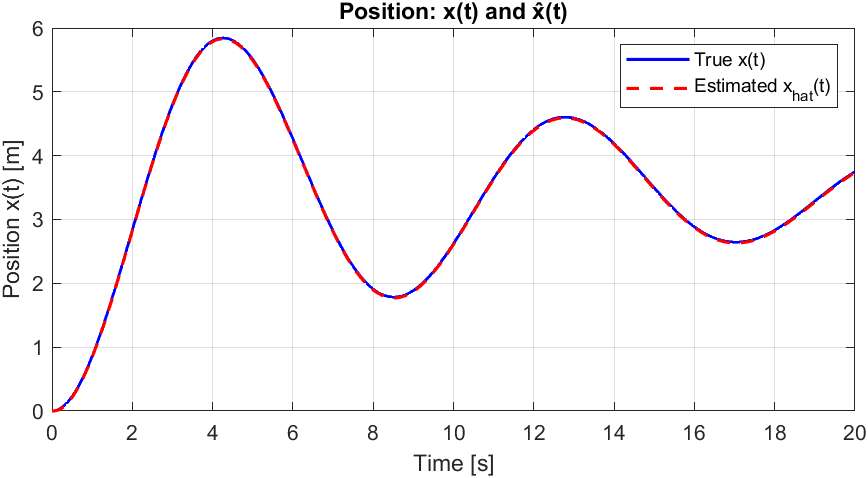
\includegraphics[width=1.1\textwidth, height=0.25\textheight]{plots/t1a_1.png}
        \caption{}
        \label{fig:t1a_1}
    \end{subfigure}
    \hfill
    \begin{subfigure}{0.45\textwidth}
        \centering
        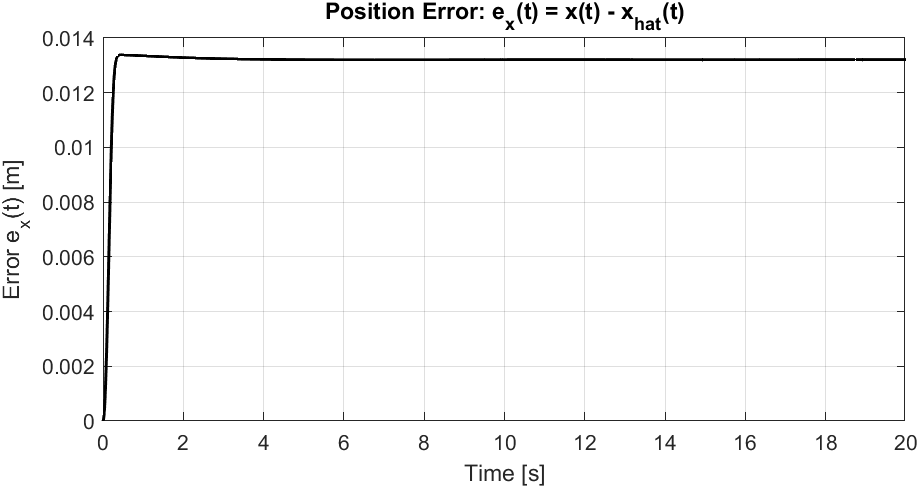
\includegraphics[width=1.1\textwidth, height=0.25\textheight]{plots/t1a_2.png}
        \caption{}
        \label{fig:t1a_2}
    \end{subfigure}
    % \hfill

\end{figure}

\begin{figure}[h!]
    % \centering
    % \hfill
    % First row
    \begin{subfigure}{0.45\textwidth}
        \centering
        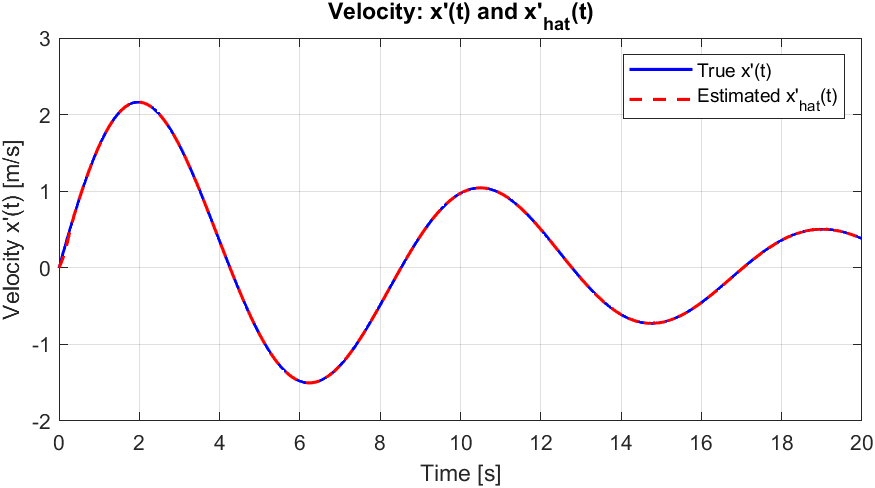
\includegraphics[width=1.1\textwidth, height=0.25\textheight]{plots/t1a_3.png}
        \caption{}
        \label{fig:t1a_3}
    \end{subfigure}
    \hfill
    \begin{subfigure}{0.45\textwidth}
        \centering
        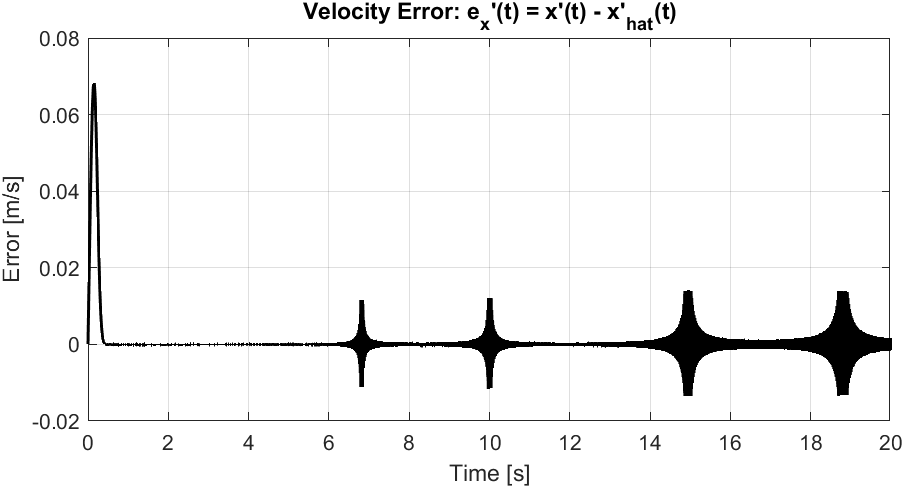
\includegraphics[width=1.1\textwidth, height=0.25\textheight]{plots/t1a_4.png}
        \caption{}
        \label{fig:t1a_4}
    \end{subfigure}
    % \hfill

\end{figure}

Υπενθυμίζουμε ότι με το φίλτρο πρώτης τάξης προέκυψε σφάλμα προς ελαχιστοποίηση το $e = \dot{x} - \dot{\hat{x}}$, με αποτέλεσμα στην πράξη να στοχεύουμε στην ελαχιστοποίηση τις διαφοράς των παραγώγων του $x(t)$ (διαφορά πραγματικού - μοντέλου). Ακόμη και σε αυτήν την περίπτωση όμως είναι φανερό ότι μπορούμε να κάνουμε αρκούντως καλές προσομοιώσεις που να έχουν μικρό σφάλμα σε σχέση με το πραγματικό μοντέλο, και αυτό οφείλετε στο fine tuning της παραμέτρου $\gamma$ (αλλά και στην επιλογή του $\lambda$, όπως και των κατάλληλων αρχικών συνθηκών). 

Βέβαια, η μικρή διαφορά στο σφάλμα δεν συνεπάγεται άμεσα και καλή εκτίμηση όλων των παραμέτρων του συστήματος. Παρακάτω παραθέτουμε τις γραφικές παραστάσεις των εκτιμήσεων αυτών για να μπορέσουμε να εξάγουμε σχετικά συμπεράσματα. (Σημαντικό για την ανάλυση των παρακάτω είναι σε κάθε διάγραμμα να κοιτάμε το scale των γραφικών παραστάσεων.)

\begin{figure}[h!]
    % \centering
    % \hfill
    % First row
    \begin{subfigure}{0.45\textwidth}
        \centering
        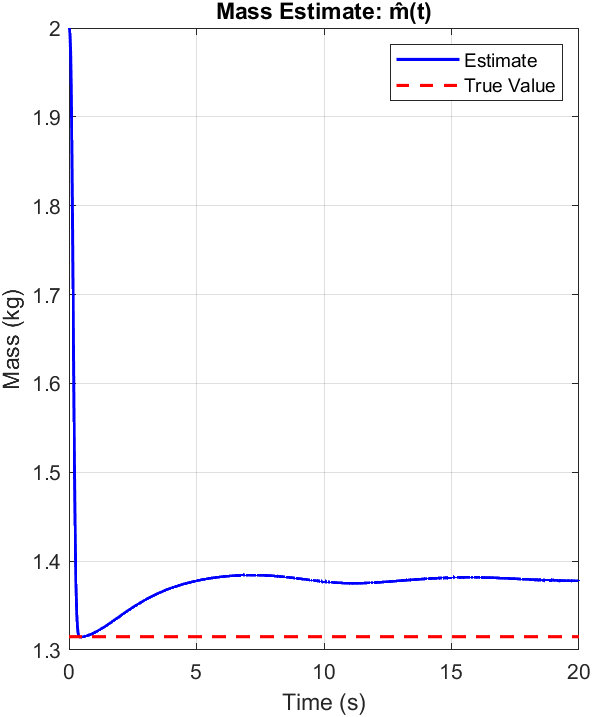
\includegraphics[width=1\textwidth, height=0.4\textheight]{plots/t1a_5.png}
        \caption{}
        \label{fig:t1a_5}
    \end{subfigure}
    \hfill
    \begin{subfigure}{0.45\textwidth}
        \centering
        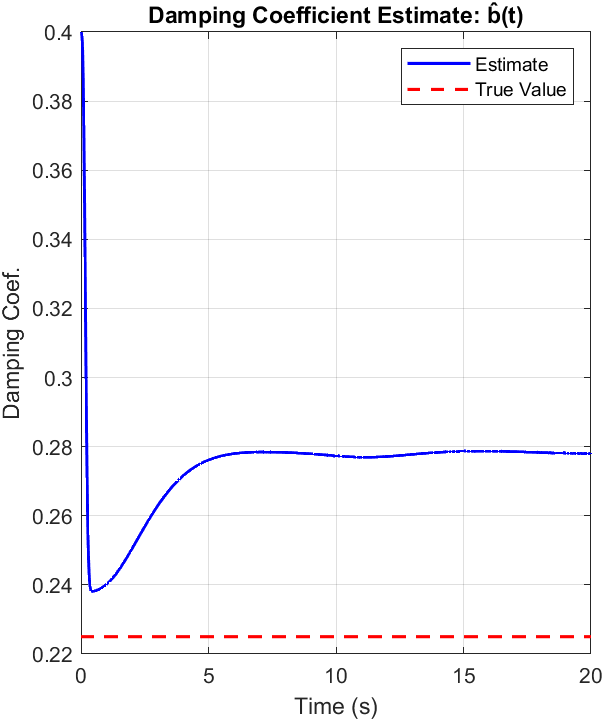
\includegraphics[width=1\textwidth, height=0.4\textheight]{plots/t1a_6.png}
        \caption{}
        \label{fig:t1a_6}
    \end{subfigure}
    % \hfill

\end{figure}

\begin{figure}[h!]
    \centering
    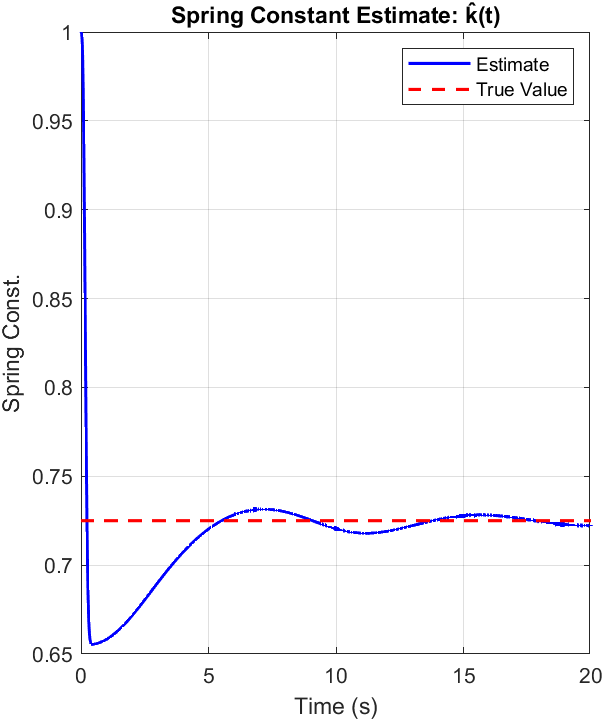
\includegraphics[width=0.47\textwidth, height=0.4\textheight]{plots/t1a_7.png}
    \caption{}
    \label{fig:t1a_7}
\end{figure}

Παρά τις προσπάθειες να καταφέρουμε να εκτιμούμε σωστά και τις τρεις παραμέτρους, πάντα τουλάχιστον μια από αυτές αποκλίνει σε αρκετά μεγαλύτερο ποσοστό από τις άλλες. Αυτό οφείλεται, μεταξύ άλλων, στην είσοδο την οποία δίνουμε για να κάνουμε την εκτίμηση (αν και σημαντικό ρόλο παίζει και το ίδιο το φίλτρο, όπως θα δούμε στην συνέχεια). Η σταθερή είσοδος (που δεν περιλαμβάνει κάποια συχνότητα), όπως θα δούμε και συγκριτικά με την ημιτονοειδή, δεν μπορεί να κάνει το ίδιο καλές εκτιμήσεις των παραμέτρων κάτι που δικαιολογείται από την Συνθήκη Επιμένουσας Διέγερσης, ΣΕΔ. Δεδομένου δηλαδή ότι έχουμε $n$ ($=3$) αγνώστους προς εκτίμηση, χρειαζόμαστε $n/2$ διαφορετικές συχνότητες για να κάνουμε ακριβή εκτίμηση σε καθεμία από αυτές.

Παρακάτω παραθέτουμε τις τελικές εκτιμήσεις των παραμέτρων, με τα σχετικά σφάλματα από τις πραγματικές τιμές τους. Πρέπει να τονίσουμε ότι ως \textit{Final estimates} ονομάζουμε όχι την τελική εκτίμηση στα $20\sec$ αλλά τον μέσο όρο των τελευταίων 5 εκτιμήσεων της κάθε παραμέτρου. Με αυτόν τον τρόπο (και σε συνδυασμό με περαιτέρω στατιστική ανάλυση\textemdash εύρεση τυπικής απόκλισης, κλπ.) μπορούμε να έχουμε μια καλύτερη/πληρέστερη εικόνα για το πού κυμαίνονται οι τιμές των εκτιμήσεων, αποφεύγοντας να πέφτουμε σε outliers.

\begin{figure}[h!]
    \centering
    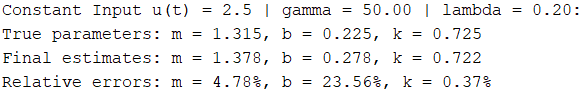
\includegraphics[width=0.6\textwidth, height=0.1\textheight]{plots/t1a_8.png}
    \caption{}
    \label{fig:t1a_8}
\end{figure}

Από τον πάνω πίνακα των logs είναι φανερό αυτό που αναφέραμε και στην ανάλυση των διαγραμμάτων των $\hat{m}(t), \ \hat{b}(t), \& \ \hat{k}(t)$, ότι δηλαδή η μία παράμετρος (σε αυτήν την περίπτωση το $\hat{b}(t)$) δεν μπορεί να εκτιμηθεί στην ίδια τάξη ακρίβειας με τις άλλες δύο). 




\begin{center}
    \textbf{(ii)} $u(t) = 2.5 \sin(t)$
\end{center}

\noindent Για την υποπερίπτωση της ημιτονοειδούς εισόδου λαμβάνουμε τα εξής αποτελέσματα:

\begin{figure}[h!]
    % \centering
    % \hfill
    % First row
    \begin{subfigure}{0.45\textwidth}
        \centering
        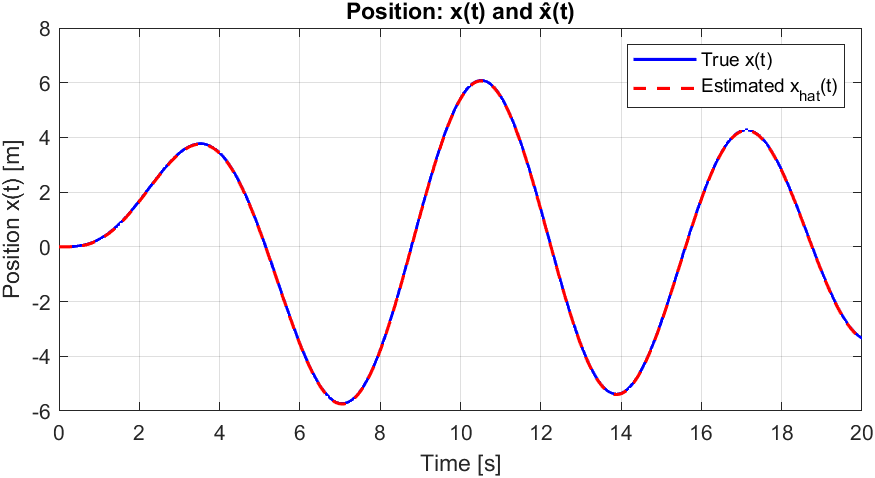
\includegraphics[width=1.1\textwidth, height=0.25\textheight]{plots/t1a_9.png}
        \caption{}
        \label{fig:t1a_9}
    \end{subfigure}
    \hfill
    \begin{subfigure}{0.45\textwidth}
        \centering
        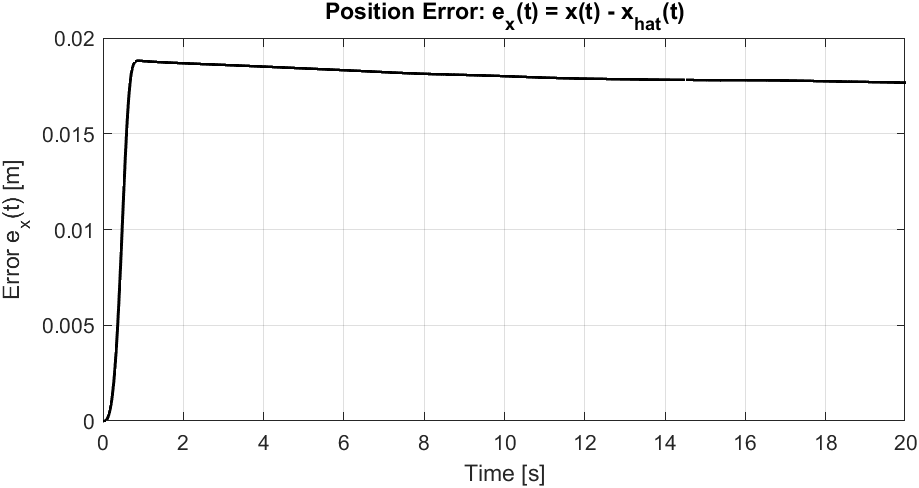
\includegraphics[width=1.1\textwidth, height=0.25\textheight]{plots/t1a_10.png}
        \caption{}
        \label{fig:t1a_10}
    \end{subfigure}
    % \hfill

\end{figure}

\begin{figure}[h!]
    % \centering
    % \hfill
    % First row
    \begin{subfigure}{0.45\textwidth}
        \centering
        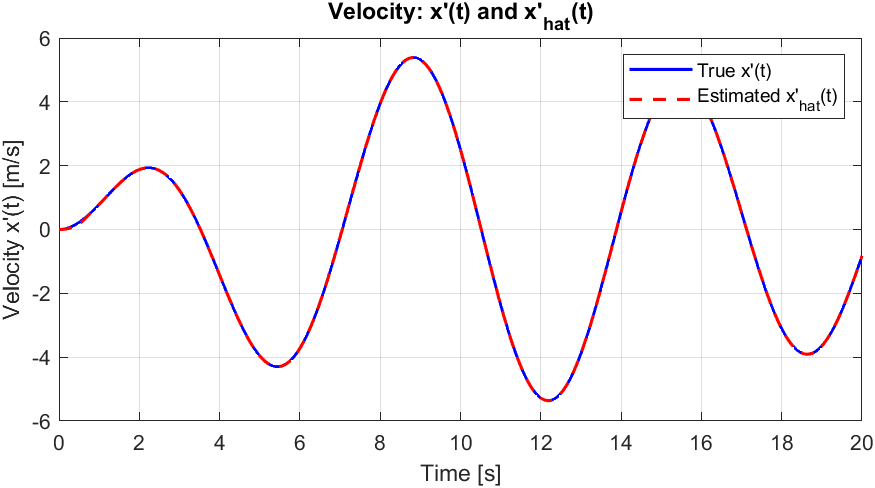
\includegraphics[width=1.1\textwidth, height=0.25\textheight]{plots/t1a_11.png}
        \caption{}
        \label{fig:t1a_11}
    \end{subfigure}
    \hfill
    \begin{subfigure}{0.45\textwidth}
        \centering
        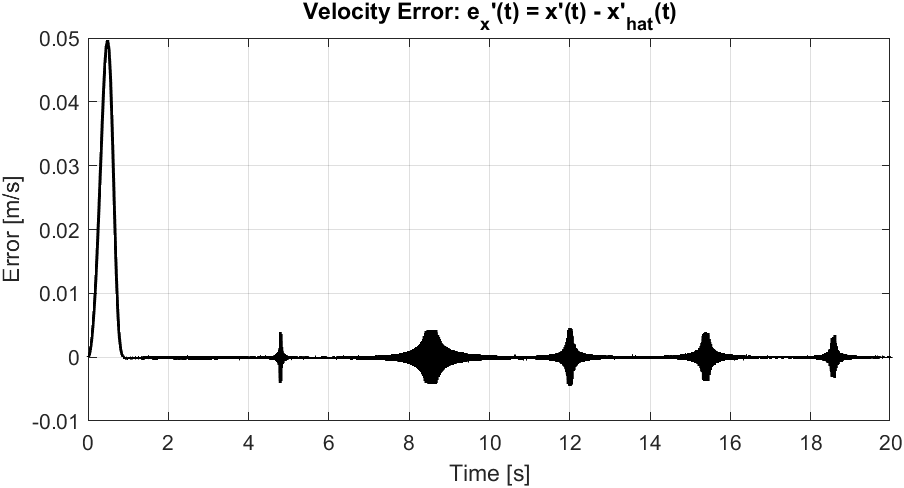
\includegraphics[width=1.1\textwidth, height=0.25\textheight]{plots/t1a_12.png}
        \caption{}
        \label{fig:t1a_12}
    \end{subfigure}
    % \hfill

\end{figure}

Συγκρίνοντας τα παραπάνω με τα διαγράμματα του υποερωτήματος (i) βλέπουμε αρχικά ότι έχουμε ελαφρώς μεγαλύτερο σφάλμα στην διαφορά $e_x = x - \hat{x}$. Παρόλα αυτά, κοιτώντας τις γραφικές παραστάσεις που αναφέρονται στο $e = \dot{x} - \dot{\hat{x}}$ (που άλλωστε αυτό ελαχιστοποιούμε), φαίνεται να έχουμε μικρότερο σφάλμα σε σχέση με την προηγούμενη περίπτωση. Η καλύτερη προσομοίωση του συστήματος οφείλεται (όπως έχουμε ήδη αναφέρει) στο γεγονός ότι πλέον δεν έχουμε ως είσοδο απλώς έναν DC όρο, άλλα ένα ημιτονοειδές σήμα (μίας συχνότητας). 

Και πάλι, για να δούμε αν όντως έχουν γίνει σωστές εκτιμήσεις όλων των παραμέτρων παραθέτουμε τις γραφικές παραστάσεις των  $\hat{m}(t), \ \hat{b}(t), \& \ \hat{k}(t)$ για να μπορέσουμε να εξάγουμε σχετικά συμπεράσματα.

\begin{figure}[h!]
    % \centering
    % \hfill
    % First row
    \begin{subfigure}{0.45\textwidth}
        \centering
        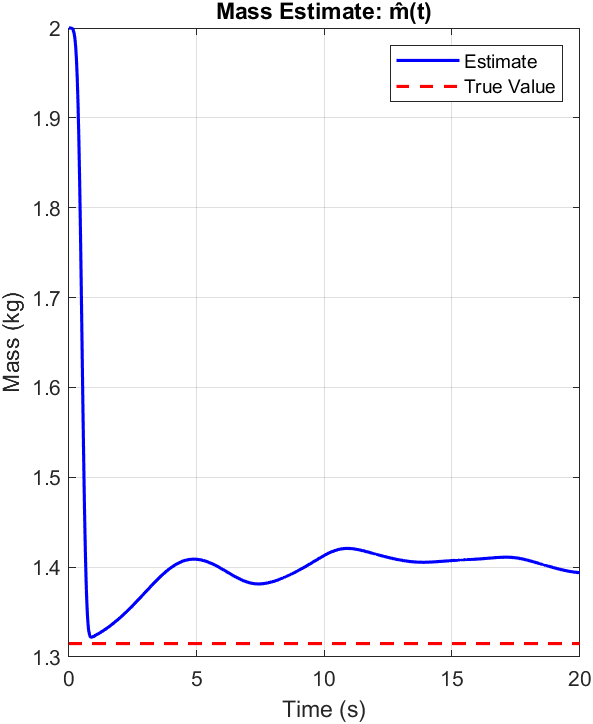
\includegraphics[width=1\textwidth, height=0.4\textheight]{plots/t1a_13.png}
        \caption{}
        \label{fig:t1a_13}
    \end{subfigure}
    \hfill
    \begin{subfigure}{0.45\textwidth}
        \centering
        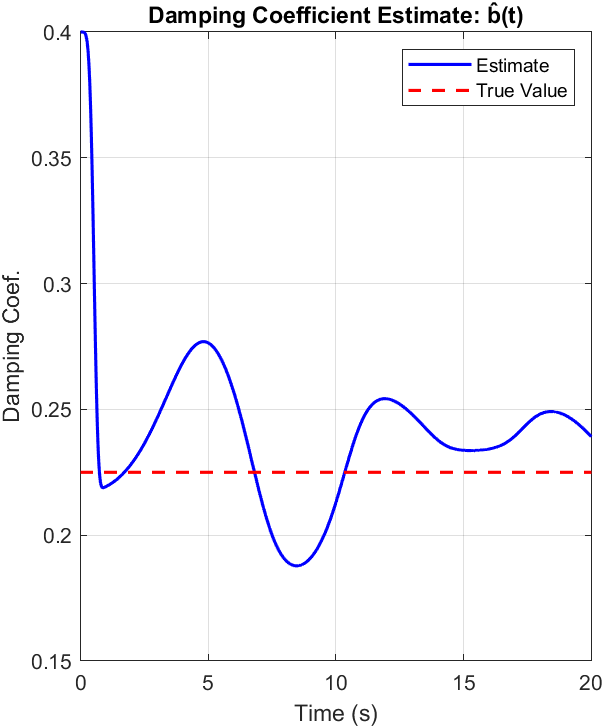
\includegraphics[width=1\textwidth, height=0.4\textheight]{plots/t1a_14.png}
        \caption{}
        \label{fig:t1a_14}
    \end{subfigure}
    % \hfill

\end{figure}

\begin{figure}[h!]
    \centering
    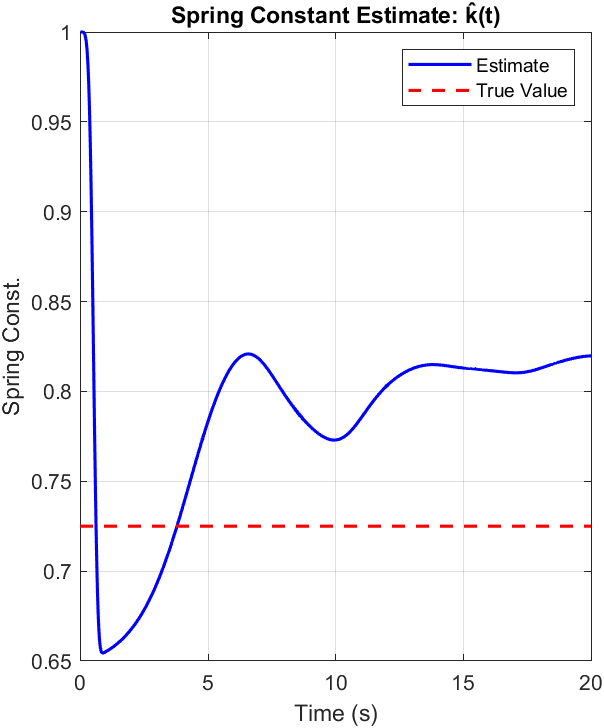
\includegraphics[width=0.47\textwidth, height=0.4\textheight]{plots/t1a_15.png}
    \caption{}
    \label{fig:t1a_15}
\end{figure}

Για συνοχή με το προηγούμενο ερώτημα κρατήσαμε τις ίδιες τιμές για τα $\gamma$ και $\lambda$ και σε αυτήν την περίπτωση εισόδου. 
Με κατάλληλο fine tuning θα μπορούσαμε να είχαμε ακόμη καλύτερα αποτελέσματα, όμως τα συμπεράσματα που εξάγουμε σε κάθε περίπτωση είναι ανάλογα, μιας και\textemdash όπως φαίνεται τόσο από το διαγράμματα όσο και από τα printed logs\textemdash πλέον τα σφάλματα των εκτιμήσεων έχουν ίδια τάξη μεγέθους (δεν υπάρχουν σημαντικές αποκλίσεις μεταξύ τους). 
Επίσης, συγκρίνοντας τον μέσο όρο των τριών σφαλμάτων για τις δύο περιπτώσεις εισόδου, βλέπουμε ότι τώρα έχουμε ελαφρώς μικρότερο μέσο σφάλμα εκτίμησης απ' ότι στην περίπτωση της DC εισόδου.
\textit{Και πάλι τονίζουμε ότι σημαντικό ρόλο στην εκτίμηση παραμέτρων παίζει και το ίδιο το φίλτρο, όπως θα δούμε στην συνέχεια.}


Παρακάτω παραθέτουμε τις τελικές εκτιμήσεις των παραμέτρων, με τα σχετικά σφάλματα από τις πραγματικές τιμές τους.

\begin{figure}[h!]
    \centering
    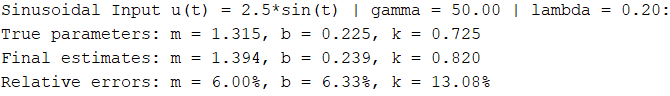
\includegraphics[width=0.6\textwidth, height=0.1\textheight]{plots/t1a_16.png}
    \caption{}
    \label{fig:t1a_16}
\end{figure}

Από τα πάνω printed logs είναι φανερό πλέον μπορούμε να διατηρήσουμε μια "ισορροπία" στα σφάλματα ώστε κανένα να μην αποκλίνει σημαντικά από από τα υπόλοιπα (και καμία παράμετρος να μην αποκλίνει σημαντικά από την πραγματική της τιμή). Γι' αυτό άλλωστε, όπως είδαμε, μπορέσαμε να ελαχιστοποιήσουμε σε μεγαλύτερο βαθμό το σφάλμα $e =  \dot{x} - \dot{\hat{x}}$ (την γραφική παράσταση) σε αυτήν την περίπτωση απ' ότι στην προηγούμενη.

\hrule

\vspace{+10pt}

\noindent\textit{\textbf{Περίπτωση Φίλτρου Δεύτερης Τάξης}} 

Για να μελετήσουμε αυτήν την περίπτωση φίλτρου θα θέσουμε:
\begin{itemize}[noitemsep, nolistsep]
    \item \texttt{filter\_version = 2}
    \item \texttt{lambda1 = 0.3}
    \item \texttt{lambda1 = 0.02}
    % \item \texttt{gamma = 1}
\end{itemize}
Εδώ η τιμή του $\gamma$ θα τεθεί διαφορετική σε κάθε ερώτημα ώστε να μπορέσουμε σε κάθε περίπτωση να δείξουμε όσο το δυνατόν πιο ακριβείς εκτιμήσεις. Πριν προχωρήσουμε, τονίζουμε ότι η επιλογή των $\lambda_1$ και $\lambda_2$ έγινε ώστε να έχουμε τους πόλους στο αριστερό ανοικτό ημιεπίπεδο (όπως είχαμε αναφέρει και στην θεωρητική ανάλυση ότι απαιτείται να ισχύει). 


\begin{center}
    \textbf{(i)} $u(t) = 2.5$
\end{center}

\noindent Για την υποπερίπτωση της σταθερής εισόδου θέτουμε \texttt{gamma = 0.001} και παίρνουμε τα παρακάτω (αυτήν την φορά δεν παραθέτουμε τις γραφικές παραστάσεις που αναφέρονται σε παραγώγους μιας και σε αυτήν την ανάλυση ελαχιστοποιούμαι το $e_x = x -\hat{x}$):

\begin{figure}[h!]
    % \centering
    % \hfill
    % First row
    \begin{subfigure}{0.45\textwidth}
        \centering
        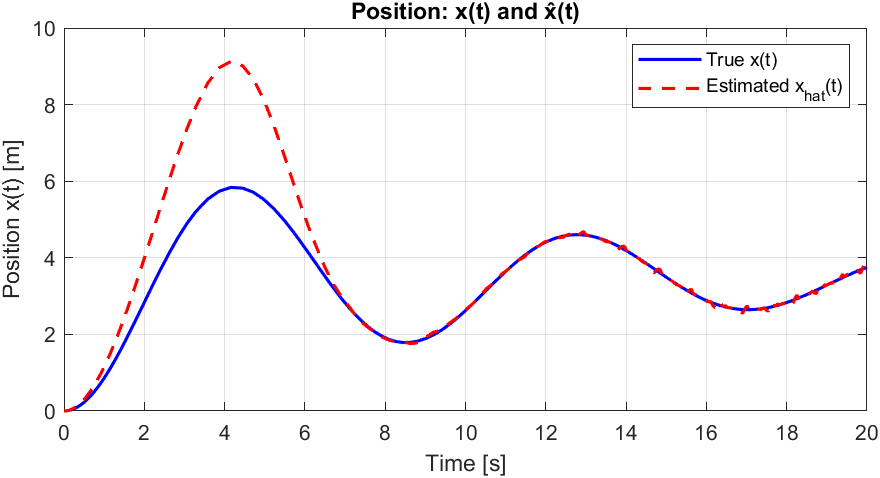
\includegraphics[width=1.1\textwidth, height=0.25\textheight]{plots/t1a_17.png}
        \caption{}
        \label{fig:t1a_17}
    \end{subfigure}
    \hfill
    \begin{subfigure}{0.45\textwidth}
        \centering
        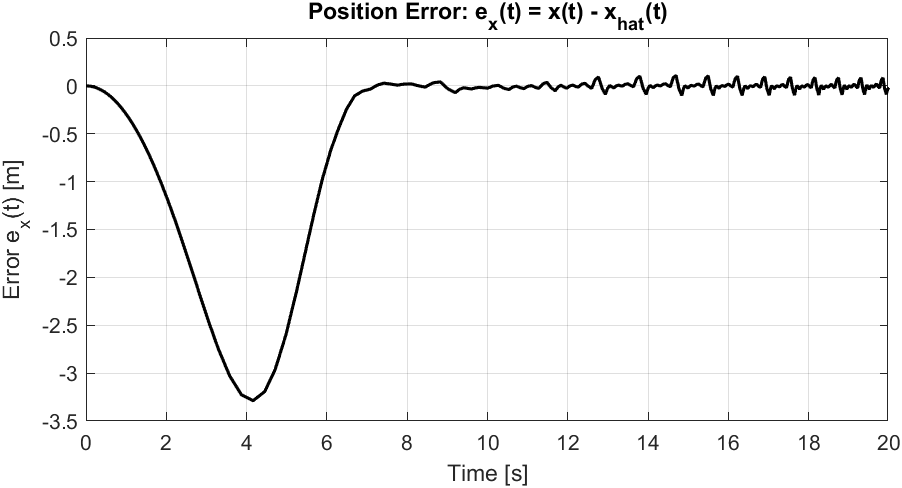
\includegraphics[width=1.1\textwidth, height=0.25\textheight]{plots/t1a_18.png}
        \caption{}
        \label{fig:t1a_18}
    \end{subfigure}
    % \hfill

\end{figure}
Εδώ, η προσομοίωση που κάνουμε δεν δίνει στην αρχή αρκετά καλά αποτελέσματα, μιας και το μικρό $\gamma$ αποτρέπει την γρήγορη αλλαγή των παραμέτρων $\hat{\theta}$ και συνεπώς και των προς εκτίμηση παραμέτρων. Ακόμη και σε αυτήν την περίπτωση όμως, εν τέλη φαίνεται το μοντέλο να μπορεί να προσαρμοστεί στα δεδομένα ελαχιστοποιώντας όσο το δυνατόν περισσότερο το σφάλμα $e_x = x -\hat{x}$.


Για να μπορέσουμε να δούμε πόσο καλά και γρήγορα εκτιμούνται οι παράμετροι που ψάχνουμε, παραθέτουμε τις γραφικές παραστάσεις των εκτιμήσεων αυτών για να μπορέσουμε να εξάγουμε σχετικά συμπεράσματα.

\begin{figure}[h!]
    % \centering
    % \hfill
    % First row
    \begin{subfigure}{0.45\textwidth}
        \centering
        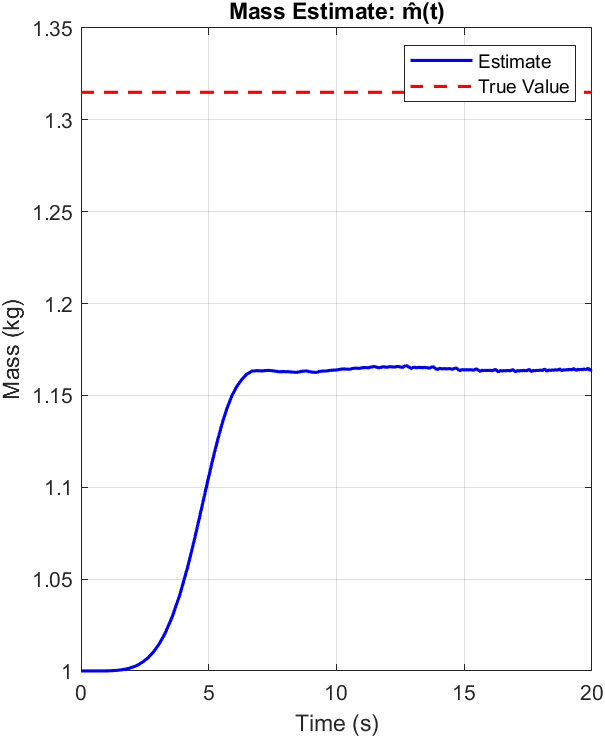
\includegraphics[width=1\textwidth, height=0.4\textheight]{plots/t1a_19.png}
        \caption{}
        \label{fig:t1a_19}
    \end{subfigure}
    \hfill
    \begin{subfigure}{0.45\textwidth}
        \centering
        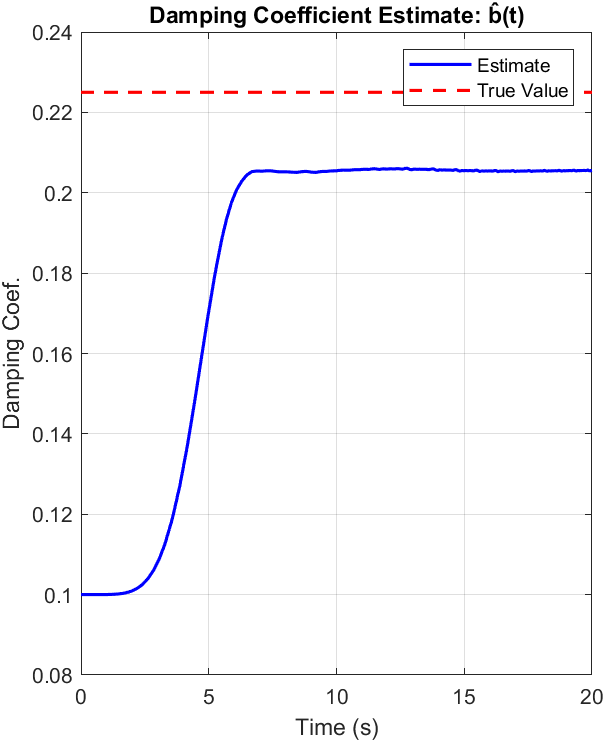
\includegraphics[width=1\textwidth, height=0.4\textheight]{plots/t1a_20.png}
        \caption{}
        \label{fig:t1a_20}
    \end{subfigure}
    % \hfill

\end{figure}

\begin{figure}[h!]
    \centering
    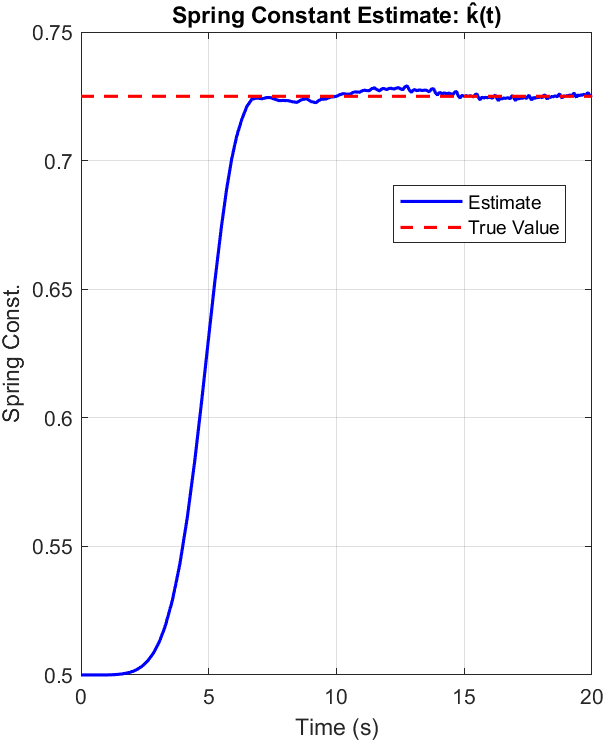
\includegraphics[width=0.47\textwidth, height=0.35\textheight]{plots/t1a_21.png}
    \caption{}
    \label{fig:t1a_21}
\end{figure}

Ένα πρώτο συμπέρασμα που εξάγουμε είναι πως και στις δύο περιπτώσεις φίλτρων, όταν βάζουμε ως είσοδο ένα DC σήμα μπορούμε να κάνουμε πολύ καλή εκτίμηση του $k$. Αυτό οφείλεται τόσο στην ίδια την ΔΕ, αλλά σημαντικό ρόλο παίζει και η επιλογή των $\lambda$ για το φίλτρο, όπως και η τιμή του $\gamma$ που επιλέξαμε.  
Και πάλι όμως, λόγω της Συνθήκης Επιμένουσας Διέγερσης, ΣΕΔ, δεν μπορούμε να κάνουμε αρκετά καλές προσεγγίσεις για όλες τις παραμέτρους που θέλουμε να εκτιμήσουμε. 

Τέλος για την υποπερίπτωση αυτή, παραθέτουμε τις τελικές εκτιμήσεις των παραμέτρων, με τα σχετικά σφάλματα από τις πραγματικές τιμές τους.

\begin{figure}[h!]
    \centering
    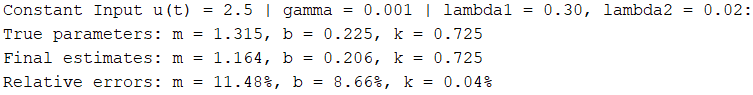
\includegraphics[width=0.7\textwidth, height=0.1\textheight]{plots/t1a_22.png}
    \caption{}
    \label{fig:t1a_22}
\end{figure}



\begin{center}
    \textbf{(i)} $u(t) = 2.5 \sin(t)$
\end{center}

\noindent Για την υποπερίπτωση της ημιτονοειδούς εισόδου θέτουμε \texttt{gamma = 1} και παίρνουμε τα παρακάτω:

\begin{figure}[h!]
    % \centering
    % \hfill
    % First row
    \begin{subfigure}{0.45\textwidth}
        \centering
        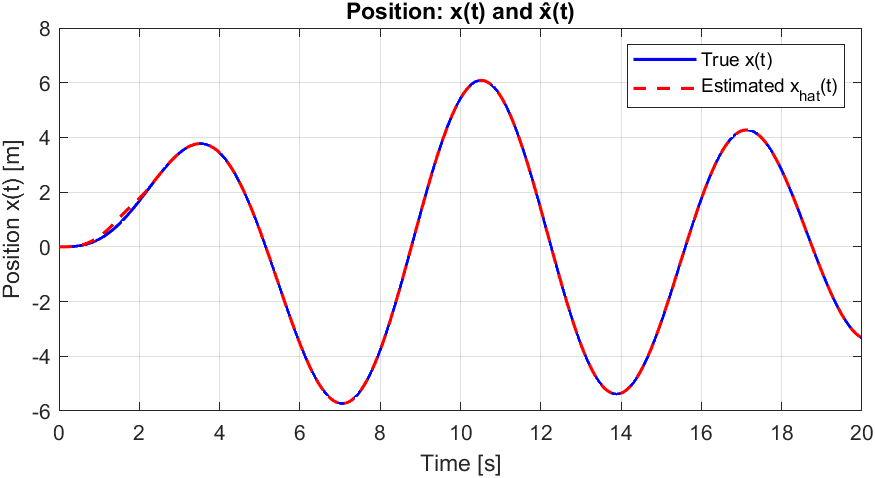
\includegraphics[width=1.1\textwidth, height=0.25\textheight]{plots/t1a_23.png}
        \caption{}
        \label{fig:t1a_23}
    \end{subfigure}
    \hfill
    \begin{subfigure}{0.45\textwidth}
        \centering
        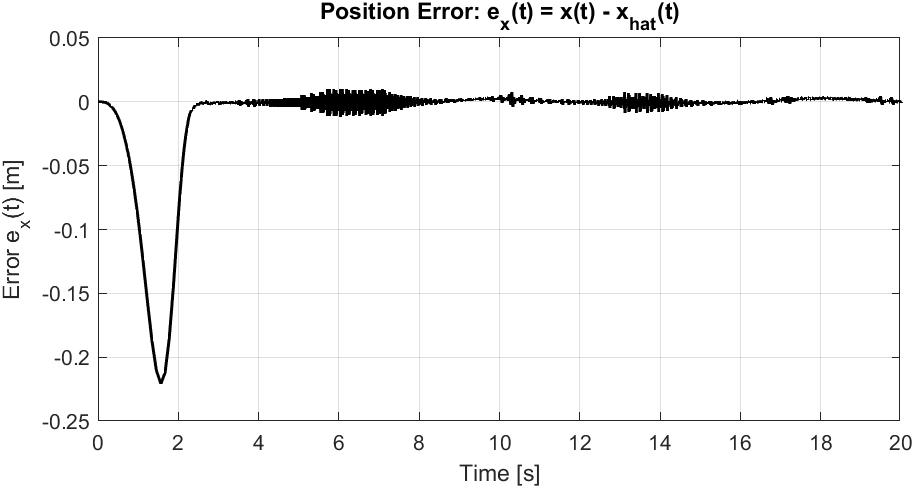
\includegraphics[width=1.1\textwidth, height=0.25\textheight]{plots/t1a_24.png}
        \caption{}
        \label{fig:t1a_24}
    \end{subfigure}
    % \hfill

\end{figure}

\vspace{-15pt}

\noindent Όπως και στις προηγούμενες προσομοιώσεις, το σφάλμα που προσπαθούμε να ελαχιστοποιήσουμε, εδώ το  $e_x = x -\hat{x}$, φαίνεται από την γραφική του παράσταση ότι όντως αποσβένει όσο περνάει ο χρόνος προς το μηδέν. Αυτό σημαίνει ότι η on-line αναδρομική μέθοδος που εφαρμόζουμε για την εκτίμηση των παραμέτρων (αν και στην θεωρία δεν είναι το ίδιο αποτελεσματική από τις off-line) μπορεί με το πέρασμα του χρόνου να κάνει όλο και καλύτερες εκτιμήσεις του συστήματος.


Για να μπορέσουμε να δούμε πόσο καλά και γρήγορα εκτιμούνται οι παράμετροι που ψάχνουμε και σε αυτήν την υποπερίπτωση, παραθέτουμε τις γραφικές παραστάσεις των εκτιμήσεων αυτών για να εξάγουμε τα σχετικά συμπεράσματα.

\begin{figure}[ht!]
    % \centering
    % \hfill
    % First row
    \begin{subfigure}{0.45\textwidth}
        \centering
        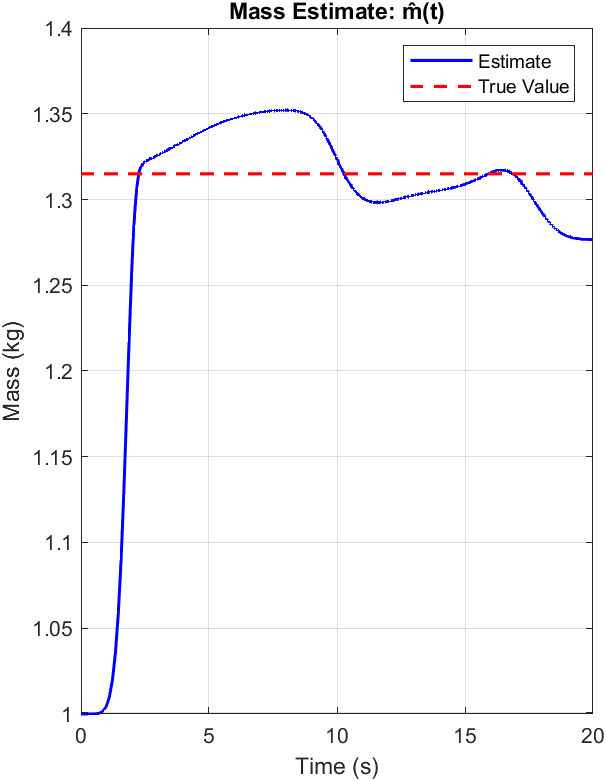
\includegraphics[width=1\textwidth, height=0.35\textheight]{plots/t1a_25.png}
        \caption{}
        \label{fig:t1a_25}
    \end{subfigure}
    \hfill
    \begin{subfigure}{0.45\textwidth}
        \centering
        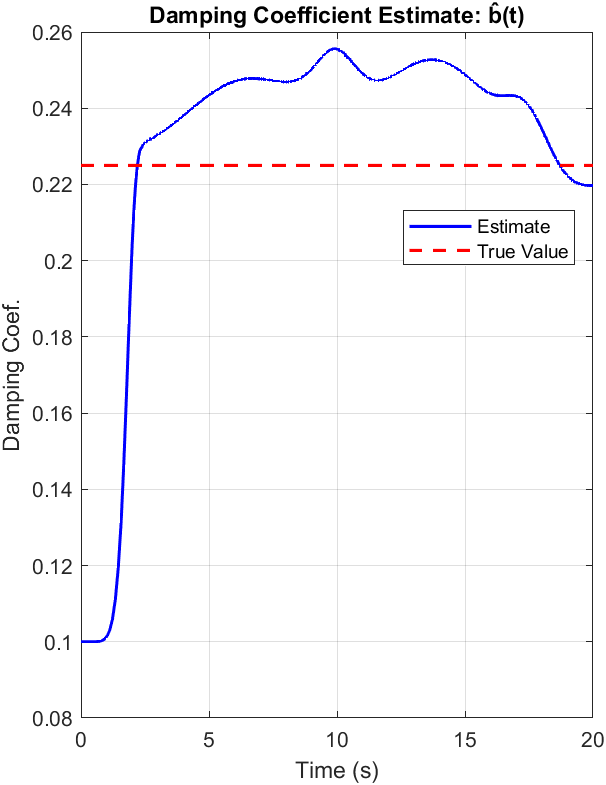
\includegraphics[width=1\textwidth, height=0.35\textheight]{plots/t1a_26.png}
        \caption{}
        \label{fig:t1a_26}
    \end{subfigure}
    % \hfill

\end{figure}

\begin{figure}[ht!]
    \centering
    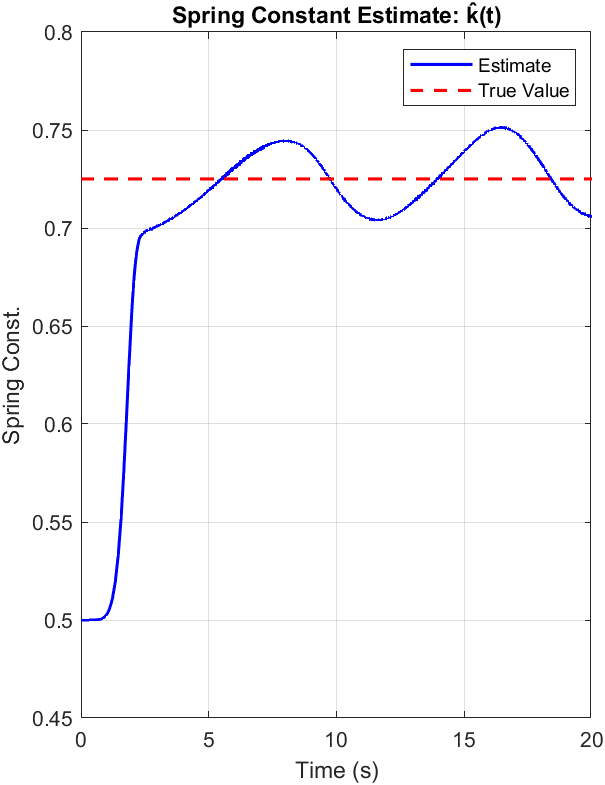
\includegraphics[width=0.47\textwidth, height=0.35\textheight]{plots/t1a_27.png}
    \caption{}
    \label{fig:t1a_27}
\end{figure}

Πλέον, παρατηρούμε ότι με το φίλτρο δεύτερης τάξης για την περίπτωση του ημιτονοειδούς σήματος μπορούμε να κάνουμε όλες τις παραμέτρους να συγκλίνουν αρκετά κοντά στις πραγματικές τους τιμές, μέσα στα $20\sec$ της προσομοίωσης. Όλα τα σχετικά σφάλματα των εκτιμήσεων, όπως φαίνονται στα printed logs, είναι περίπου ίδια και μικτότερα από όλες τις προηγούμενες περιπτώσεις (κατά μέσο όρο). Συμπεραίνουμε ότι ο συγκεκριμένος συνδυασμός εισόδου και φίλτρου είναι ο ιδανικότερος για την εκτίμηση των παραμέτρων μας (σε σύγκριση πάντα με τις προηγούμενες περιπτώσεις που αναφέρθηκαν). 

\begin{figure}[ht!]
    \centering
    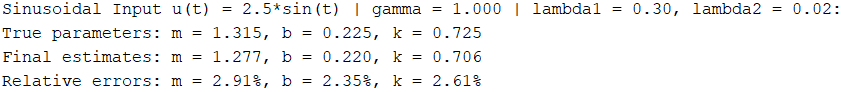
\includegraphics[width=0.8\textwidth, height=0.12\textheight]{plots/t1a_28.png}
    \caption{}
    \label{fig:t1a_28}
\end{figure}

\vspace{+100pt}



\newpage




\end{document}
